  \documentclass[12pt]{article}
%\usepackage{fancyhdr,minitoc}
\usepackage{graphicx}
\usepackage{hyperref}
\usepackage[dvipsnames]{xcolor}
\usepackage{ulem}
%\usepackage{psfig}

\usepackage{times}
%\usepackage{mathptm}
\def\void#1{{}}
\voffset=-2.5cm
\hoffset=-2.5cm 
\topskip=0.5cm 
\textwidth=17.0cm
\textheight=23.5cm
%
\usepackage{natbib}
\usepackage{aas_macros}
\bibpunct{(}{)}{;}{a}{}{,}
%\citestyle{aa}
%
%%%%%%%%%%%%%%%%%%%%%%%%%%%%%%%%%%%%%%%%%%%%%%%%%%
\begin{document}

%%%%%%% Setting param/commands


\newcommand{\lp}{\textit{LePHARE++} }
\newcommand{\zphot}{ $z_\mathrm{phot}$ }
\newcommand{\tbd}{ {\color{Cyan}[TBD]} } 
\newcommand{\comment}[1]{ {\color{Magenta}[#1]} }


%\psdraft
\noindent  
\begin{table}[h]
\centering
\begin{tabular}{|c|}
\hline
\  \\
\Huge  {\bf Le PHARE++} \\
\  \\
\Large {\ \ \ \ \ \ \ \ \ \ \ \  PHotometric Analysis for \ \ \ \ \ \ \ \ \ \ \ \ }\\
\Large {\ \ \ \ \ \ \ \ \ \ \ \   Redshift Estimations    \ \ \ \ \ \ \ \ \ \ \ \ }\\
\  \\
\hline
\end{tabular}
\end{table}
\vspace*{0.5cm} \\
\large
\centerline{ St\'ephane ARNOUTS \& Olivier ILBERT} \\
\centerline{Laboratoire d'Astrophysique de Marseille}\\
\centerline{ \ \ } \\
\large
\centerline{Johann COHEN-TANUGI } \\
\centerline{Laboratoire Univers et Particules de Montpellier}
\vspace*{0.5cm} 
%
%
\begin{center}
With the contribution of Iary Davidzon, Mara Salvato, C\'edric Dubois, Emeric Le Floc'h, Raphael Shirley, and Maria Petkova
\end{center}
\vspace*{0.5cm} 
\normalsize
\tableofcontents
%
\newpage
%


%%%%%%%%%%%%%%%%%%%%%%%%%%%%%%%%%%%%%%%%%%%%%%%%%%%%%%%%%%%%%%%%%%%%%%
\section{Getting started}\label{sect:starter}
%%%%%%%%%%%%%%%%%%%%%%%%%%%%%%%%%%%%%%%%%%%%%%%%%%%%%%%%%%%%%%%%%%%%%%
%
%
%
%%%%%%%%%%%%%%%%%%
\subsection{Introduction}\label{subsect:introduction}
%%%%%%%%%%%%%%%%%%
%
%
\lp is a set of \texttt{C++} programs to compute
 photometric redshifts (\zphot) for galaxies and AGN, and galaxy physical parameters\footnote{If BC3-like templates are used, \zphot and galaxy physical parameters can be computed at the same time} by fitting spectral energy distributions (SEDs) to a dataset of photometric fluxes or apparent magnitudes.  Stellar templates are fitted too.
 It is based on the previous Fortran version of \textit{LePHARE}, a code described 
 in Arnouts et al. (1997) and Ilbert et al. (2006).
 % Not convinced that it should be here. Many more papers than that. TBD. \textcolor{blue}{and widely used since then (e.g., Salvato et al. 2009, Ilbert et al. 2010, Salvato et al 2011, Ilbert et al. 2013, Dahlen et al. 2013, Mobasher et al. 2015, Santini et al. 2015, Hsu et al 2014, Ananna et al 2017}.
 \lp package is composed of four parts:
 \begin{itemize}
 \item a preliminary step to read the SED and build the SED library;
 \item a preliminary step to read the  input filters set and build the filter library ;
 \item a program to compute apparent magnitudes in the filter set for each template of the library,
 along a grid of redshift, adding dust attenuation and nebular emission lines and storing the results. 
 This step  allows the user to  extract  basic information relative to 
  the filters (e.g.~$\lambda_{mean}$, AB-corrections, attenuation)
  and SEDs (e.g.~k-corrections, color-color diagrams, etc.). 
 \item  The photometric redshift code based on a  $\chi^2$ fitting method. This part can also be used to compute physical parameters.
\end{itemize}


% In addition, the suite provides a code to generate realistic, multicolor catalogs, taking into account observational effects. There are also graphic tools to plot \lp outputs. \tbd  \comment{Iary: Put other general comments here. Or acknowledgement like ``if you use this code for your work please cite ''... } \citet{Arnouts1999,Ilbert2006}
%
%
%%%%%%%%%%%%%%%%%%%%%%%%
\subsection{Download and installation}\label{subsect:installation}
%%%%%%%%%%%%%%%%%%%%%%%%
%
The basic package is available from the website:  \url{http://still.to.be.done.fr}.
Each file is briefly described in Appendix A. Additional SED libraries (in separate tarballs) are also available on the same webpage. \\
\\
Before starting, you must set two environment variables:
\begin{itemize}
\item \texttt{\$LEPHAREDIR} is the root directory of the software (e.g., \texttt{/home/yourname/LEPHARE/})
\item \texttt{\$LEPHAREWORK} is the path of a new directory which will be created when compiling the code (e.g.~\texttt{\$LEPHAREDIR/work/}). \texttt{\$LEPHAREWORK} will contain libraries created by \lp (it can be placed anywhere). 
The code will use \texttt{\$LEPHAREDIR/work/} if it doesn't exist.
\end{itemize}
These two environment variables could be set definitively in the usual files depending on your shell (e.g., \texttt{.bash\_profile} or \texttt{.csh\_envlph}) as any environment variable. \\
 
Once downloaded (and unpackaged) \lp, enter in the directory \texttt{source}. Then open the file \texttt{Makefile} and modify its options according to your OS if needed (see notes below). \\
\\
Once your OS is ready to compile the code, execute the commands:\\
\$ make clean\\
\$ make\\
if you recompile once again from scratch. 
Note that the directory \texttt{\$LEPHAREWORK} will be created during this phase. \\
You can create the directory \texttt{\$LEPHAREWORK} separately with the command:\\
\$ make work\\

You can use \texttt{Makefile} to build a gzipped file containing all the source files by the command:\\
\$ make archive
\\

%Another use of \texttt{Makefile} is\\
%\$ make archive\\
%to build a gzipped file containing all the source files.\\


Notes on the compiler options:\\
 With the default set-up, the compiler is GNU \texttt{g++} with basic 
optimization flags (\texttt{-g -std=c++11 -O3}). If you want to enable parallelization (OPENMP), other options should be included (e.g., \texttt{-lpthread}). MacOS users must be aware that the \texttt{g++} installed via XCode is a wrapper of \texttt{clang} and can raise errors while compiling; the easiest solution is to install the original GNU compiler (in the GCC package by Free Software Foundation) available through Homebrew or MacPorts. Note also that the code has been tested with GCC versions $>6$ (6.3.0 and 7.3.0); older versions may result in critical errors.     

\subsection{Example with one run}

We provide an example of the whole procedure for a test catalog included in the package in \\ \texttt{\$LEPHAREDIR/test/}.
For this example, we used the COSMOS2015 catalogue (Laigle et al. 2016)  but limited to the zCOSMOS bright sample, for which also spectroscopy is provided. You can find more detailed examples in \texttt{\$LEPHAREDIR/examples/}. Different configurations are tested, showing how to configure the code for this application. All the key steps are considered.

%%%%%%%%%%%%%%%%%%%% 
\subsection{Structure}

 The structure of the package is illustrated in Fig~\ref{fig:skim}. 
 Each step is described in the following sections. First, one has to define the filters used in the input galaxy catalog (program \texttt{filter}). The other initial step is constructing a library of rest-frame galaxy SEDs from synthetic models or observed spectra (program \texttt{sedtolib}). Then, another program builds a grid of apparent magnitudes at different redshifts, adding dust attenuation and nebular emission lines to each SED in the library (program  \texttt{mag\_gal}). The main \lp program (program \texttt{zphota}) will use the file containing such a grid to fit the photometry from the input catalog.
% If we enumerated the steps in the introduction, we could write: following the opening, with step 1, we do this, in step 2, this is happening, etc.
 

%\begin{figure} 
%\psfig{figure=lephare_skim.pdf,angle=0,width=16.cm,clip=}
%\caption{Illustration of the package structure} 
%\label{fig:skim}
%\end{figure} 
\begin{figure} 
\resizebox{\hsize}{!}{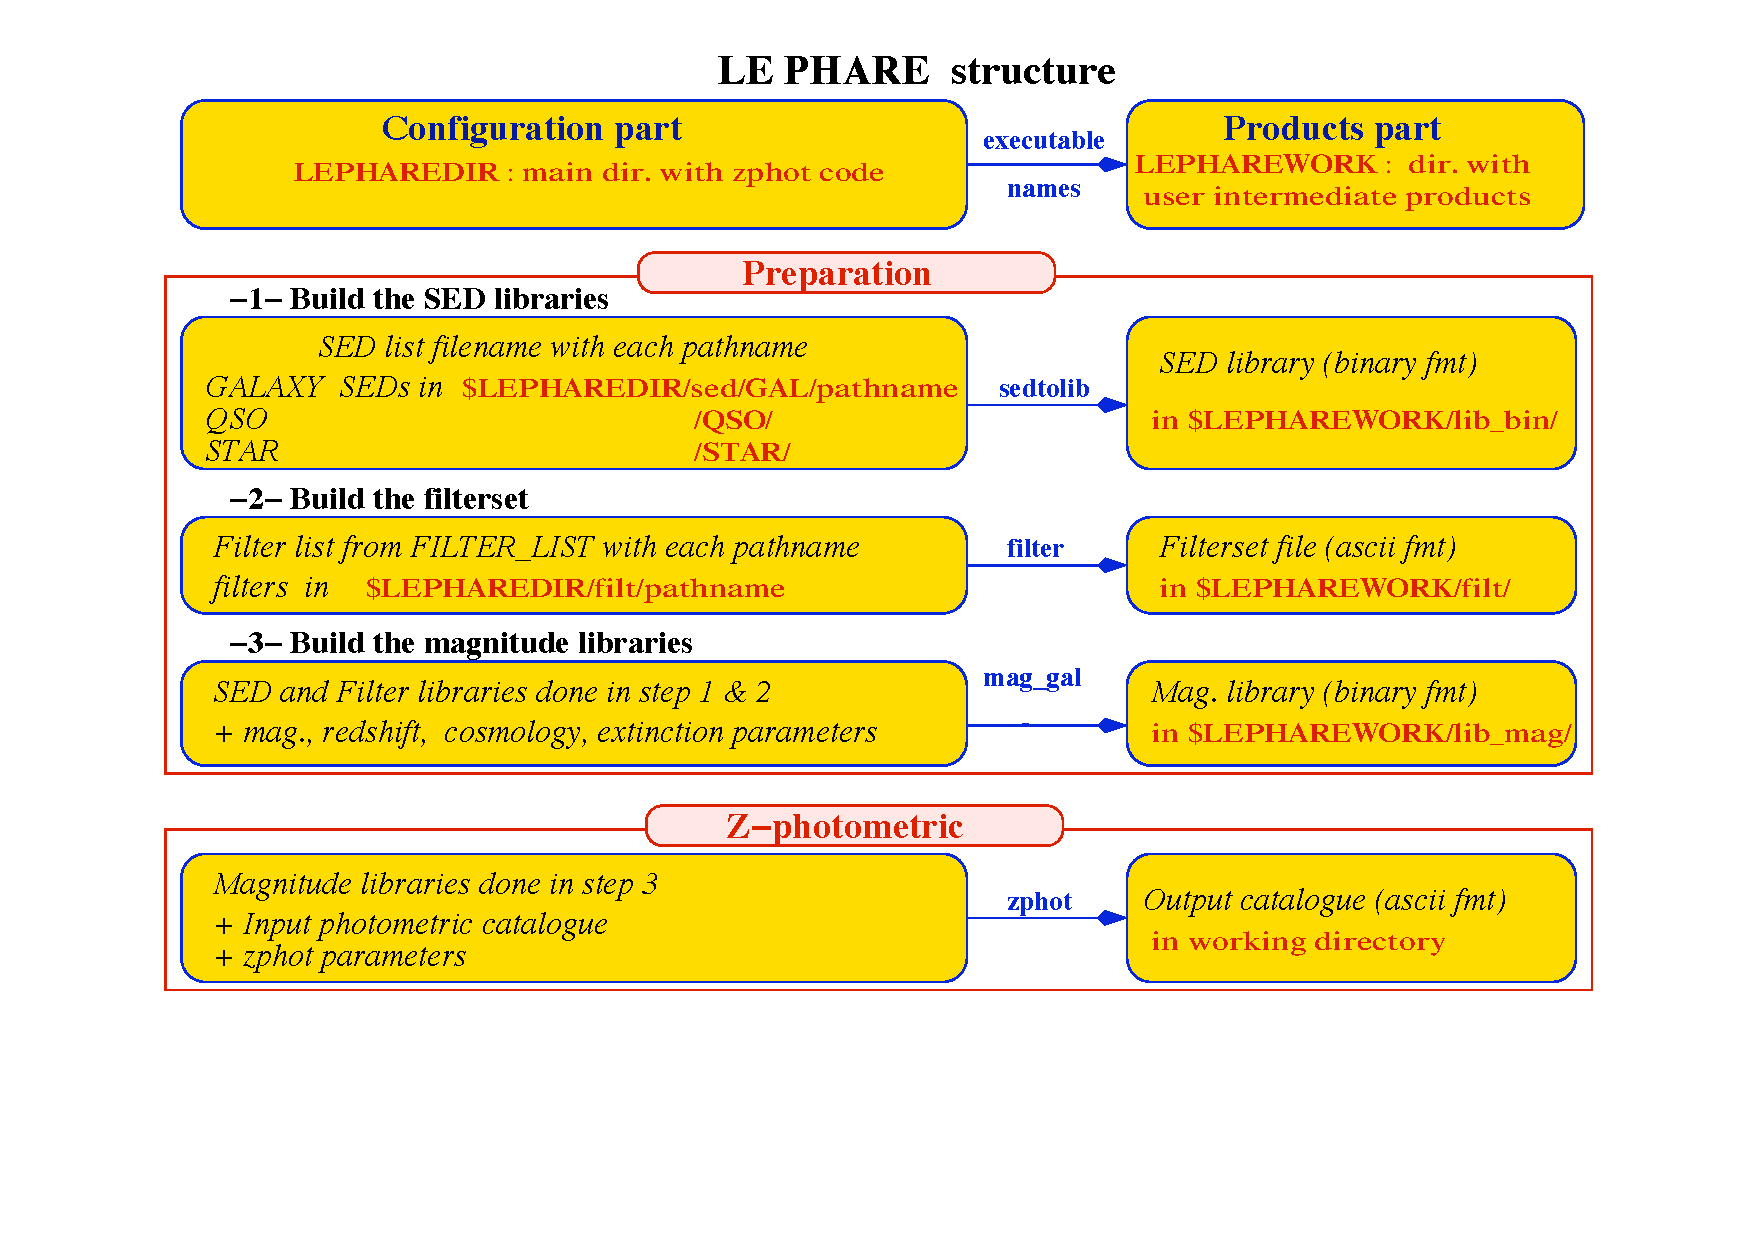
\includegraphics{lephare_skim}}
%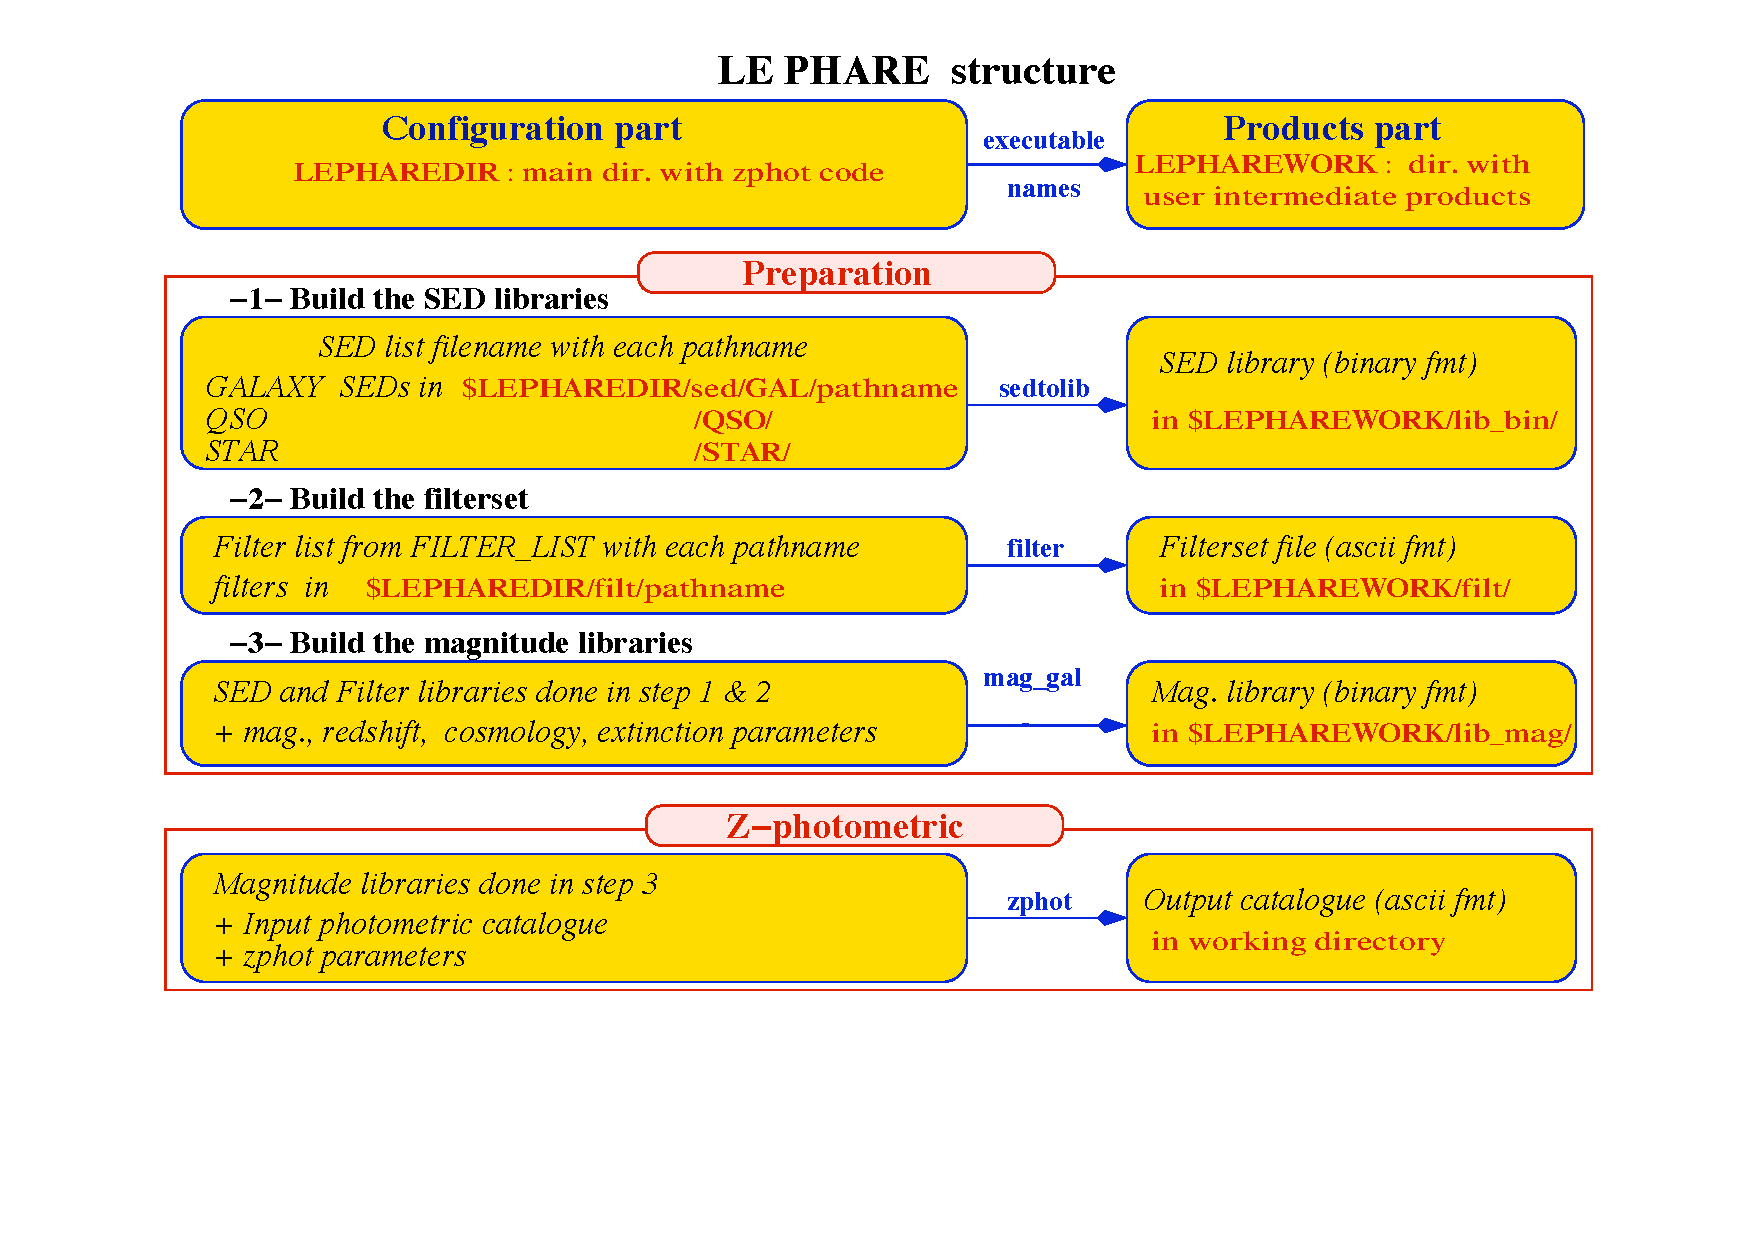
\includegraphics[width=21cm]{lephare_skim}
\caption{Illustration of the package structure } 
\label{fig:skim}
\end{figure} 

%
%%%%%%%%%%%%%%%%%%%%
\subsection{Syntax}

 All the programs in the suite can be run from a Unix shell with the following
 syntax: \\
%
\$  $<$program$>$ -c  $<$configfile$>$ [ -Parameter {\it value}...] \\
%
 where $<$program$>$ is the name of the program, followed by a
 configuration file called with the  {\bf -c } option. The various code options are defined in this file but can also be given through additional instructions in the command line. Using such an optional list of parameters, any {\bf -Parameter}~{\it value} statement overrides the values in the configuration file.  
 % A help message can be printed with the option -h or - -help \tbd.

 The parameters associated with the various programs can be included in a single configuration file (e.g., \texttt{zphot.para}) 
 % except the simulation program. 
 You can store your parameter file where you want (e.g., in the directory where you run the code or in \texttt{\$LEPHAREDIR/config/}) to keep configuration files of different runs.  
Configuration files must be in ASCII format, compliant with the following rules: 
%
\begin{itemize}
\item Only one parameter per line, 
with the syntax: PARAMETER\_NAME  value(s)
\item Comment line starts with ``\#''.
\item Depending on the parameter, values can be  Float, Integer, or String (without quotation marks). 
\item When a parameter accepts multiple values, these must be comma separated (no space).
\item When a parameter accepts a file location (as a String), the path can include environmental variables (\texttt{\$HOME} and \texttt{\$LEPHAREDIR}). 
\item Some parameters are mandatory, \lp will print out an error message if they are not set (either in the configuration file or via the command line)
\item Other parameters can be omitted (\lp will assign a default value to them)
\end{itemize}
%
In the next sections, we will mark the mandatory parameters with an asterisk  ("*"). \\

You can use the option \texttt{VERBOSE NO} if you don't want that \texttt{mag\_gal} and \texttt{zphota} display the template or sources computed. It could be helpful if run in batch mode. 

%\textcolor{red}{Somewhere, we need to have the list of parameters set by default with their default value. The alternative is to provide a complete zphot.para file listing all the possible parameters. Probably, we are already doing this. We need to add a few sentences about it here.}
 
 \newpage
 
 
%%%%%%%%%%%%%%%%%%%%


%%%%%%%%%%%%%%%%%%%%
\section{Rest-frame SED libraries through  \texttt{sedtolib}}\label{models}
%
%
\subsection{Overview}
%  string list_keywords[] =  {"t","GAL_SED","GAL_FSCALE","GAL_LIB","SEL_AGE","AGE_RANGE","QSO_SED","QSO_FSCALE","QSO_LIB","STAR_SED","STAR_LIB","STAR_FSCALE"};

A set of libraries for stars, galaxies, and quasars are available in \$LEPHAREDIR/sed/STAR, \$LEPHAREDIR/sed/GAL, \$LEPHAREDIR/sed/QSO\footnote{A more appropriate name for the directory would be AGN, but QSO is kept for compatibility reasons with original work.} directories and organized in different sub-folders.
  
Each sub-folder contains a specific collection of SED files, described in a README (how those SEDs were built, etc.), and a file (usually with the suffix \texttt{.list}) listing the relative path of the SED files to be used as input for \texttt{sedtolib}.  
For STAR and QSO and most of the galaxies, SEDs are written in  ASCII, with  $\lambda(\AA)$, flux[$erg/s/\AA/cm^2$], with increasing $\lambda$\footnote{$F_\lambda$ or F does not matter, as a normalization will be applied.}.
For Galaxy, in addition to empirical SEDs, output files from stellar synthesis population models (Pegase and BC03) with a more complex format can also be used by adding a specific character after the file name in the SED list file (see end of section 2.2.2). 
% 
%
\subsection{ \texttt{sedtolib} program }
  The program {\bf sedtolib} is used to build the different STAR, QSO 
   and GALAXY libraries from a list of SED files.
%
  The goal of this program is to generate from different kinds of SEDs (star/AGN/galaxy)
   with various original formats (ASCII, binary), a unique binary file with direct access
    that can be easily read in the following steps.
   The binary output file (*.bin) is saved in the directory \${\it LEPHAREWORK}/lib\_bin/ 
   with an attached doc file (*.doc) and a file with physical information (*.phys) for galaxies.
   The new SED format is ($\lambda(\AA)$,flux[$erg/s/\AA/cm^2$]).   
    For models with input SEDs expressed in  luminosity or energy ($L_{\odot}/\AA$,$\nu L_{\nu}$,...),
    like PEGASE, GISSEL, or the FIR libraries, the SED are converted in flux ($erg/s/cm^2/\AA$). 

\subsubsection{Syntax and parameter values}
 
 Specific parameters have been duplicated for 
 the STAR, QSO, and GAL(axy) categories with different names to simplify this algorithm section. The option -t allows you to specify 
 if galaxy (G), star (S), or QSO (Q) parameters have to be read.  \\
%
The syntax is: \\

$\%$ {\bf sedtolib} -t G [or Q or S]  -c zphot.para \\

 
%\begin{table}[h]
\begin{tabular}{lccl}
\hline
 parameter     & type    & default &  description \\
\hline
 XXX\_SED(*)    & string  & ---- & Full pathname of file with the list of selected SED files  \\
                         & (n=1)   &      &                                               \\
%
 XXX\_LIB(*)    & string  & ---- & Name of the output binary library (with no extension) \\
                        & (n=1)   &      & Files {\it \$XXX\_LIB}.bin, {\it  \$XXX\_LIB}.doc and 
                                                  {\it  \$XXX\_LIB}.phys      \\
                        &             &      & saved in   \${\it LEPHAREWORK}/lib\_bin/       \\
%
 XXX\_FSCALE  & float   & 1.0  & Flux scale to be applied to each SED in the list \\
              & (n=1)   &      &                                                  \\
%
 SEL\_AGE   & string  & NONE &  Full pathname of file with a list of ages (Gyr)  \\
                     &  (n=1)  &            &   to be extracted from GISSEL or PEGASE SEDs. \\
%
AGE\_RANGE& float  &  ----- &  Range of age (Gyr)   \\

                      & (n=2) &        &            \\


\hline
\end{tabular}\\

The extracted text from zphota.para, related to the {\bf sedtolib} task.The parameter value "XXX" means either GAL or QSO or STAR. Note that SEL\_AGE and AGE\_RANGE are relevant only when using templates including an age (e.g. BC03). \\



\subsubsection{Building libraries  from a list of SEDs }  

The easiest is to take a  predefined list of SED  in the existing subdirectories and look at the README file.  \\
 
 \noindent \underline{For stars  (\$LEPHAREDIR/sed/STAR)}, SEDs are available in the subdirectories : \\
  $\bullet$  PICKLES/:   131 stellar SEDs from Pickles (1998)    \\
  $\bullet$  BD/:  Low mass stars library from Chabrier et al. (2000)  \\
  $\bullet$  BD\_NEW/:  Brown dwarfs library from Baraffe et al. 2015, Morley et al. 2012, 2014  \\
   $\bullet$ LAGET/: (missing REF)\\
  $\bullet$  WD/:  4 white dwarfs from Bohlin et al. (1995) \\
  $\bullet$  SPEC\_PHOT: Spectro-Photometric standards from Hamuy et al. (1992, 1994)\\
 
 
  \noindent \underline{For QSOs  (\$LEPHAREDIR/sed/QSO)},  there is a 
   list of observed spectra from different authors and some synthetical QSOs listed in the subdirectory (synth/). In particular, a list of templates was successfully used for computing the photometric redshift of the {\it XMM} and {\it Chandra} AGN identified in COSMOS.  In short, the library includes pure QSO and hybrid templates obtained by combining galaxies with various AGN and QSO templates with different relative ratios. The details of the template construction are outlined in Salvato et al. (2009). Note that, unlike for galaxies, the templates to be used in QSO depend on the type of AGN and QSO to be fitted (see Salvato et al 2011, Fotopoulou et al. 2012, Hsu et al. 2014, Ananna et al. 2017)\\
    
  \noindent \underline{For galaxies (\$LEPHAREDIR/sed/GAL)}, SEDs are available in the following subdirectories: \\
  %$\bullet$  42GISSEL/ :  42 SEDs  with a single age extracted from GISSEL96  \\
  $\bullet$  CFHTLS\_SED/: 66 SEDs used for CFHTLS photo-z paper (Arnouts et al. 2007)  \\
  $\bullet$  COSMOS\_SED/: 31 SEDs used for COSMOS photo-z paper (Ilbert et al. 2009, 2013, Salvato et al. 2011, Dahlen et al. 2013)  \\ 
  $\bullet$  CWW\_KINNEY/: original CWW  and Kinney spectra \\
  %$\bullet$  POGGIANTI/:   8 SEDs \\
  %$\bullet$  VIRGO/:   10 SEDs from VIRGO cluster analysis (Boselli et al.) \\
  %$\bullet$  GISSEL/:  list of SEDs with GISSEL96 \\
  $\bullet$  BC03\_CHAB/:  SEDs from the BC03 library. These templates are derived with exponentially declining Star Formation Histories.\\
  $\bullet$  BC03\_CHAB\_DELAYED/:  SEDs from the BC03 library. These templates are derived with delayed Star Formation Histories.\\
  %$\bullet$  PEGASE2/ :  list of SEDs with  PEGASE2 library \\
   
  \noindent \underline{For Far-Infrared (FIR) SEDs (\$LEPHAREDIR/sed/GAL)}, different SEDs are available :\\
  $\bullet$   CHARY\_ELBAZ/:  105 FIR templates for different luminosity \\
  $\bullet$   DALE/ : 64 FIR templates \\
  $\bullet$   LAGACHE/:  46 FIR templates \\
  $\bullet$  SK06/ :  different set of starburst models based on Siebenmorgen \&Krugel (2006)\\
  Note that for the first 3 libraries (CHARY-ELBAZ, DALE, LAGACHE),
   we have subtracted a stellar component from their SEDs to get only the dust contribution at the shortest wavelengths.  \\
  
\noindent To know the format of the SEDs that are used in your list, an additional character must be specified after each SED file, allowing you to mix in one list of different types of galaxy SEDs. 
 For example, you could prepare a new list which includes: \\
BC03\_CHAB/bc2003\_lr\_m52\_chab\_tau03\_dust00.ised\_ASCII  BC03 \\
BC03\_CHAB/bc2003\_lr\_m62\_chab\_tau03\_dust00.ised\_ASCII  BC03\\
COSMOS\_SED/Ell1\_A\_0.sed \\
COSMOS\_SED/Ell2\_A\_0.sed   \\

\noindent In each list, it is possible to comment a template with \#.    \\
 
\noindent For ASCII SED file, no character is required. The character %{\bf P} is used for PEGASE2 models,
{\bf BC03} is used for the Bruzual and Charlot 2003 models. For the BC03 templates, the file is in ASCII for the C++ version of LePhare, to avoid the problem of portability between various systems.   \\
  For the list with FIR SEDs,  the character {\bf LW} (as for Long Wavelength) is required.  
 
 
\subsubsection{Physical information for the galaxies }  

For the galaxy templates, an additional file is generated by the program {\texttt{sedtolib}} with some physical properties (*.phys). This information will be used when running the photo-z code to derive physical parameters. It contains the following parameters:  \\
   Model   Age    $L_{UV}$    $L_R$   $L_K$   $L_{IR}$   Mass   SFR   Metallicity   Tau    $D_{4000}$    \\
  where \\
Age is expressed in yr \\
$L_{UV}$ is NUV monochromatic luminosity (Log([erg/s/Hz])) ($\int_{2100}^{2500} L_{\lambda} d\lambda /400 * 2300^2/c$ )) \\
$L_R$ is optical r monochromatic luminosity (Log([erg/s/Hz])) ($\int_{5500}^{6500} L_{\lambda} d\lambda /1000 * 6000^2/c$ ))\\
$L_K$ is NIR    K monochromatic luminosity  (Log([erg/s/Hz])) ($\int_{21000}^{23000} L_{\lambda} d\lambda /2000 * 22000^2/c$ ))\\
$L_{IR}$ is the IR luminosity (Log([$L_{\odot}$])) \\
Mass is the stellar mass ($M_{\odot}$), .i.e. the mass truly in stars (not the integral of the SFH) \\
SFR is the ongoing star formation rate ($M_{\odot}/yr$) \\
Metallicity is  the Gas metallicity of the galaxy \\
Tau is the e-folding parameter for a star formation history with SFH=exp(-t/tau)   (yr) \\
$D_{4000}$ is the 4000A break measured as in Bruzual 1983 ($D_{4000}= \int_{4050}^{4250} F_{\lambda} d\lambda / \int_{3750}^{3950} F_{\lambda} d\lambda$) \\
If not available, the parameters are set to -99. \\

The IR luminosity ($L_{IR}$)  is derived using LW libraries. For the Infra-red libraries ( LW: Dale, Lagache, Chary-Elbaz, Siebenmorgen \& Krugel) the IR luminosity is measured from 8 to 1000 microns. These luminosities may be slightly different then the ones quoted by the authors due to the different definitions of the $L_{IR}$ integration limit and because (at least for Dale, Lagache, and Chary-Elbaz) we have subtracted the underlying stellar component from the original SEDs.\\

%$\bullet$ For the Pegase models (F) the IR luminosity is given as input  if internal extinction is applied \\
%$\bullet$ For the stochastic Bruzual and Charlot library ( BC\_STOCH ), the IR luminosity is estimated 
     

\subsubsection{Adding libraries}

New SEDs can be easily added to the current ones.
 They must be located in the appropriate directory (GAL/STAR/QSO).
  If they are ASCII files they must be in $\lambda(\AA)$, flux[$erg/s/\AA/cm^2$], with increasing $\lambda$.
%New BC03 or PEGASE models can be included if the format did not changed.
    
  
  \subsection {example}
 
  
\noindent  {\bf sedtolib  -t} G  {\bf -c} zphot.para {\bf -GAL\_SED}  \$LEPHAREDIR/sed/GAL/CFHTLS\_SED/CFHTLS\_MOD.list  {\bf -GAL\_LIB}  LIB\_CFHTLS  \\
 %
  This command reads the list of galaxy templates given by the keyword {\bf -GAL\_SED}  (as indicated by {\bf -t} G).  \\
  A binary file LIB\_CFHTLS.bin with a LIB\_CFHTLS.doc and LIB\_CFHTLS.phys  files are saved in \$LEPHAREWORK/lib\_bin/. \\

\noindent  {\bf sedtolib -t} S {\bf -c} zphot.para {\bf -STAR\_SED}  \$LEPHAREDIR/sed/STAR/STAR\_MOD.list {\bf -STAR\_LIB}   LIB\_STAR \\
%
This command reads the list of star templates given by the keyword  {\bf -STAR\_SED}  (as indicated by {\bf -t} S). \\
A binary file  LIB\_STAR.bin and a  LIB\_STAR.doc file are saved in \$LEPHAREWORK/lib\_bin/. \\
  

\noindent  {\bf sedtolib -t} Q {\bf -c} zphot.para {\bf -QSO\_SED}  \$LEPHAREDIR/sed/QSO/QSO\_MOD.list {\bf -QSO\_LIB}   LIB\_QSO \\
%
This command reads the list of QSO templates given by the keyword  {\bf -QSO\_SED}  (as indicated by {\bf -t} Q). \\
A binary file  LIB\_QSO.bin and a  LIB\_QSO.doc file are saved in \$LEPHAREWORK/lib\_bin/. \\

An example of a misleading command:\\
\noindent  {\bf sedtolib -t} S {\bf -c} zphot.para {\bf -GAL\_SED}  \$LEPHAREDIR/sed/GAL/CWW\_KINNEY/CWW\_MOD.list   {\bf -GAL\_LIB}   LIB\_CWW \\
%
This command will work and will read the galaxy templates given by  {\bf -GAL\_SED} but will interprete them as stars rather than galaxies because the option is set to S: {\bf -t  S} !
 \\

% NOT HERE. IN mag_gal. \textcolor{blue}{For all the example above, there is the option to save the output of {\bf sedtolib} in ASCII  with the command --LIB\_ASCII YES. The file will be saved in the working directory. The file can be used for creating evolutionary tracks of templates, color changes due to extinction etc.}

The parameters passed in the command line can also be changed in the configuration (zphot.para) file, except -t and -c.
 \newpage
%
%%%%%%%%%%%%%%%%%%%%


%%%%%%%%%%%%%%%%%%%%
\section{Filters }
\label{sec:filter}
%

Several sets of filters, from different telescopes, are available in the directory \texttt{\$LEPHAREDIR/filt/}. You could find most of the standard filters (like the Johnson-Kron-Cousins in \texttt{filt/jkc}). New set of filters can be added there.

By default, the filters are stored in \texttt{\$LEPHAREDIR/filt/}, but you could change this repository using the keyword \texttt{FILTER\_REP}. With this keyword, you could indicate if you prefer to store the filters in another directory.

\subsection{Description and outputs}

The  program {\bf filter} puts  together a list of filter response curves, 
 and applies some transformations  according to the nature of the filters. 
 The resulting file in the directory \${\bf LEPHAREWORK/filt/}.\\
% Additional programs ({\bf filter\_info} and {\bf filter\_extinc}) can be used to get  more information about the filters.  
 
\subsection{Syntax and parameter values}
 The syntax is : $\%$ {\bf filter -c}  zphot.para \\
%
 The following parameters  are considered: \\
\small
%\begin{table}[h]
\begin{tabular}{lccl}
\hline
 Parameters     & type    & default &  description \\
\hline
FILTER\_REP    & string       & \$LEPHAREDIR/filt/ & Name of the repository containing the filters.  \\ 
                            & (n$=$1)   &     \\
FILTER\_LIST(*)& string       & ---- & filter files separated by a comma. \\
                           & Nfilt not limited &     &   \\ 
%
 TRANS\_TYPE    & float         & 0  & Filter transmission type: 0= Energy; 1= Photon    \\
                             & n=1 or n=Nfilt &    &   \\
%
 FILTER\_CALIB  & integer     & 0    & Filter calibration for long wavelengths  [0-def].    \\
                            & n=1 or n=Nfilt &     &   \\
                            %                                                                               
 FILTER\_FILE   & string       & filter & Name of the file with all combined filters . \\ 
                            & (n$=$1)   &      &  It is saved in \${\bf LEPHAREWORK/filt/}.\\

\hline
%
\end{tabular}
%\end{table}  
%
\normalsize
\subsection{Parameter descriptions}
\label{sec:filter}
\noindent {\bf FILTER\_LIST} : all the filter names must be separated by a comma.
    We assume that all the filter files are located in the  directory {\bf \$LEPHAREDIR/filt/}, except if the keyword {\bf FILTER\_REP} is specified.
    When writing the set of filters to be used,  only the 
    pathname after the common string {\bf \$LEPHAREDIR/filt/} should be specified. \\

\noindent {\bf TRANS\_TYPE} : 
 Type of the transmission curve for each filter, separated by a comma. 
 The number of arguments should match the number of filter but if only value is given,
  which will be use for all the filters. \\ 
  %
 The transmissions ($T_{\lambda}$)   are dimensionless (in \% ), however they refer 
 either to a  transmission in Energy or Photon which will slightly modify the
 magnitude estimates. 
  The magnitude is :
  \[ mag(*) = -2.5 \log_{10} \frac{\int F_{\lambda}(*) R_{\lambda} d\lambda}{\int F_{\lambda}(Vega) R_{\lambda} d\lambda}  \] 
 %
 If the transmission curve ($T_{\lambda}$)  corresponds to energy then $R_{\lambda}=T_{\lambda}$, \\
%
 If the transmission curve ($T_{\lambda}$) corresponds to number of photons ($N_{\varphi}$) then $R_{\lambda}= \lambda T_{\lambda}$ : 
% 
\[ N_{\varphi} =  \frac{ F_{\lambda} d\lambda }{h\ \nu} = \frac{F_{\lambda} \lambda d\lambda }{h\ c} \rightarrow  
 mag(*)=-2.5 \log_{10} \frac{\int F_{\lambda}(*) \lambda T_{\lambda} d\lambda}{\int F_{\lambda}(Vega) \lambda T_{\lambda} d\lambda}  \rightarrow  R_{\lambda}=\lambda T_{\lambda}  \]
%
 When building the filter library, the filter shape is changed with respect to the original one as
 follows :
 \[ R_{\lambda}=T_{\lambda} ( \frac{\lambda}{< \lambda >})^{tt} \],
  where $tt$ is the value of  TRANS\_TYPE parameter and  $< \lambda >$ is the mean
  wavelength of the filter. \\
%
The modification of filter shape can be significant for long wavelength filters and when the filter is broad.  Nevertheless it is often not the dominant source of errors with respect to other uncertainties relative to QE-CCD, telescope transmission, atmospheric extinction shape etc... \\
 In the output filter file specified by the keyword {\bf FILTER\_FILE}, we save the values  
 ($\lambda (\AA)$,$R_{\lambda}$). \\
%
 
\noindent {\bf FILTER\_CALIB} : This keyword allow to consider specific calibrations at long 
 wavelengths  in order to apply a correction factor to the original flux estimated by  LEPHARE
 (see section~\ref{sec:filtcalib} for more details). \\
%
 We define the correction factor as
 fac\_corr$=\frac{\int  R_{\nu} d\nu}{\int \frac{B_{\nu}}{B_{\nu_0}} R_{\nu} d\nu}= \frac{\int  R_{\lambda} d\lambda/\lambda^2}{1/\lambda_0^2 \int \frac{B_{\lambda}}{B_{\lambda_0}} R_{\lambda} d\lambda}$, where
 $B_{\nu}$ is the reference spectrum used to calibrate the filters and  $\lambda_0$ is  the effective wavelength defined as  $\lambda_{0}= \frac{\int R_{\lambda} B_{\lambda} \lambda d\lambda}{\int R_{\lambda}  B_{\lambda}  d\lambda}$.\\
 %
The value of {\bf FILTER\_CALIB} allows to describe different combinations of $\nu_0$
 and $B_{\nu}$: \\
  \noindent {\bf FILTER\_CALIB= 0} : $\frac{B_{\nu}}{B_{\nu_0}}=1$ or $B_{\nu}=ctt$. 
                              This is the default value used in LEPHARE. \\
  \noindent {\bf FILTER\_CALIB= 1} : $\nu B_{\nu}=ctt$.  This describes the SPITZER/IRAC, ISO calibrations\\
  % NO IDEA \textcolor{red} {what about WISE?}.  \\
  \noindent {\bf FILTER\_CALIB= 2} : $B_{\nu}=\nu$. This describes the sub-mm calibrations.\\
  \noindent {\bf FILTER\_CALIB= 3} : $B_{\nu}=$black body at T=10,000K. \\
  \noindent {\bf FILTER\_CALIB= 4} : A mix calibration with $\nu_0$ defined from
                                                          $\nu B_{\nu}=ctt$ and  the flux estimated as 
                                                          $B_{\nu}=$black body at T=10,000K.  This appears
                                                          to be  the  adopted scheme for the SPITZER/MIPS calibration.\\ 
  \noindent {\bf FILTER\_CALIB= 5} : Similar mix calibration with   $\nu_0$ defined from
                                                           $\nu B_{\nu}=ctt$ and the flux estimated as $B_{\nu}=\nu$. 
                                                           This may reflect the SCUBA calibration.                              
%
\subsection{Filter informations} 
%
\subsubsection{Standard filter informations} 
 As an example, using  default values listed in the configuration file zphot.para. \\
\begin{tabular}{ll} 
\hline
FILTER\_LIST     &  tmp/f300.pb,tmp/f450.pb,tmp/f606.pb,tmp/f814.pb,tmp/Jbb.pb,tmp/H.pb,tmp/K.pb \\
TRANS\_TYPE    &    0                                                                        \\
FILTER\_CALIB  &    0                                                                        \\
FILTER\_FILE    &    HDF.filt                                                               \\
\hline \\
\end{tabular}
%
%
 Run the program :$\%$ {\bf filter -c} zphot.para. \\
  It generates the file HDF.filt  by combining all  filters and saved it in \${\it LEPHAREWORK}/filt. \\
  It  returns informations about the filters on screen. 
  Another stand alone program allows also to read informations about existing filter list 
  (with $\%$ {\bf filter\_info  -f}  HDF.filt).  \\
  The following informations are written on the screen : \\
  \\
\noindent
\begin{tabular}{lcrrrrrrr|rrr}
\#NAME&ID&$\lambda_{mean}$&$\lambda_{eff}^{Vega}$& FWHM & ABcor& TGcor&VEGA&  $M_{\odot}^{AB}$& CAL &   $\lambda_{0}$ &  Fac \\
F300W&1 & 0.2999 & 0.2993 & 0.0864 & 1.398&99.99 & -21.152 & 7.433 &0& 0.2999 & 1.000  \\
F450W&2 & 0.4573 & 0.4513 & 0.1077 &-0.074&-0.339& -20.609 & 5.255 &0& 0.4573 & 1.000  \\
F606W&3 & 0.6028 &0.5827  &0.2034  &0.095 & 0.161 &-21.367 & 4.720 &0& 0.6028 & 1.000  \\
F814W&4 & 0.8013 &0.7864  &0.1373  &0.417 & 0.641 &-22.322 & 4.529 &0& 0.8013 & 1.000  \\
Jbb      &5 & 1.2370 &1.2212  &0.2065  &0.890 & 99.99 &-23.748 & 4.559 &0& 1.2370 & 1.000  \\
H        & 6 & 1.6460 &1.6252  & 0.3377 & 1.361& 99.99 &-24.839 & 4.702 &0& 1.6460 & 1.000  \\
K        & 7 &  2.2210& 2.1971 & 0.3967 & 1.881& 99.99 &-26.012 & 5.178 &0& 2.2210 & 1.000\\
\end{tabular}
%
\\
where : \\
 Col 1 : Name put in the first row of the filter file \\
 Col 2 : incremental number \\
% Col 3 : ``Area'' of the filter in $\AA$ : $ \int R_{\lambda} d\lambda$ \\
 Col 3 : Mean wavelength ($\mu m$) : $ \int R_{\lambda} \lambda d\lambda / \int R_{\lambda} d\lambda $ \\ 
 Col 4 : Effective  wavelength with Vega ($\mu m$) : $ \int R_{\lambda} F_{\lambda}(Vega)\lambda d\lambda / \int R_{\lambda}F_{\lambda}(Vega) d\lambda $ \\
 Col 5 : Full Width at Half of Maximum ($\mu m$) \\
 Col 6 : AB Correction where $m_{AB} = m_{VEGA} + ABcor$ \\
 Col 7 : Thuan Gunn correction where $m_{TG} = m_{VEGA} + TGcor$. (99.99 if undefined) \\
 Col 8 : VEGA magnitude :    $2.5\log_{10}(\int R_{\lambda} F_{\lambda}(Vega) d\lambda / \int R_{\lambda} d\lambda$)\\
 Col 9 : AB absolute magnitude of the sun ($M^{AB}_{\nu,\odot}$) \footnote{ convertion from absolute magnitude to luminosity: by combining the
           distance modulus  ($m-M=5log D[pc]-5$) and the luminosity ($L_{\nu}[erg.s^{-1}.Hz^{-1}]= A\pi D^2[cm^2] f_{\nu}[erg.s^{-1}.cm^{-2}.Hz^{-1}]$)
           you get:  $L_{\nu,\odot}[erg.s^{-1}.Hz^{-1}]=10^{-0.4(M^{AB}_{\nu,\odot} -51.605)}$    }\\
 Col 10: value of the calibration used for ($B_{\nu}/B_{\nu_0}$,$\nu_0$) in {\bf FILTER\_CALIB} \\
 Col 11: Effective  wavelength ($\mu m$)  $\lambda_{0}^{B_{\nu}}= \frac{\int R_{\lambda} B_{\lambda} \lambda d\lambda}{\int R_{\lambda}  B_{\lambda}  d\lambda}$.\\
 Col 12: Correction factor to be applied to the original flux measured by LEPHARE. 
             This correction is included in the programs {\bf mag\_gal} and {\bf mag\_star} as
             $flux^{cor}= flux^{LePhare}\times$fac\_cor \\ 
%
%\newpage
\subsubsection{Extinction informations}

 The stand alone program ({\bf filter\_extinc}) returns information about  atmospheric extinctions and galactic extinctions.\\
  A set of atmospheric extinction curves  and  galactic extinction laws are
  available in \$LEPHAREDIR/ext/ directory.   
 It includes Calzetti and Prevot extinction laws. The Cardelli law is hardcoded in the programs and is the default law for the galactic extinction. \\

%

\% {\bf filter\_extinc}  -c COSMOS.para   -FILTER\_FILE filter\_test.dat\\
 It returns: \\ 
\#\#\#\#\#\#\#\#\#\#\#\#\#\#\#\#\#\#\#\#\#\#\#\#\#\#\#\#\#\#\#\#\#\#\#\#\#\#\#\\
\# Computing ATMOSPHERIC AND GALACTIC EXTINCTION \\
\# with the following options: \\
\begin{tabular}{ll}                       
\# Filters: & filter\_extinc.dat\\
\# Atmospheric extinction curve: & extinc\_etc.dat\\
\# Galactic extinction curve: & CARDELLI\\
\# Output file: & filter\_extinc.dat\\
\end{tabular}                 \\
\#\#\#\#\#\#\#\#\#\#\#\#\#\#\#\#\#\#\#\#\#\#\#\#\#\#\#\#\#\#\#\#\#\#\#\#\#\#\#\\

\begin{tabular}{lccc}  
 Filters & Ext(mag/airmass) & Albda/Av & Albda/E(B-V)      \\
         cosmos/u\_cfht   &  0.486  &    1.504  &    4.663  \\
       cosmos/B\_subaru   &  0.264  &    1.297  &    4.020  \\
       cosmos/V\_subaru   &  0.141  &    1.006  &    3.118  \\
       cosmos/r\_subaru   & 0.096   &    0.858  &    2.659  \\
       cosmos/i\_subaru   & 0.052   &    0.643  &    1.992  \\
cosmos/suprime\_FDCCD\_z  & 0.027   &    0.471  &    1.461  \\
                vista/Y   & 0.049   &    0.391  &    1.211  \\
                vista/J   & 0.096   &    0.281  &    0.871  \\
                vista/H   & 0.100   &    0.181  &    0.562  \\
                vista/K   & 0.100   &    0.118  &    0.364  \\
\end{tabular}\\
%where : \\
Col 2 : Mean atmospheric extinction  (mag/airmass) using (EXT\_CURVE): $A_{\lambda}= \int R_{\lambda} Ext(\lambda) d\lambda / \int R_{\lambda} d\lambda $ \\
 $Ext(\lambda)$ comes from any atmospheric extinction curve that is put in \${\it LEPHAREDIR}/ext/.   \\
Col 3 : Mean galactic attenuation (in $A(\lambda)/A_V$) using  the
  galactic extinction law (GAL\_CURVE). 
Col 4 : Mean galactic attenuation (in $A(\lambda)//E(B-V)$)  as a function
 of color excess (E(B-V)) assuming $A_V=R_V\times E(B-V)$.  \\

  For $R_V$ coefficients, we assume  $R_V=3.1$ for most extinction laws but 
   Calzetti ($R_V=4.05$) and Prevost ($R_V=2.72$).\\    
  Others extinction laws can be added by  following the format  ($\lambda(\AA) , k_{\lambda}$).   \\ 
\begin{figure} 
%\includegraphics[width=7cm]{Gal_extinction}
\caption{Exemple of attenuation ($A_{\lambda}/E(B-V)$) for different filters in UV wavelength (GALEX :FUV, NUV and FOCA)  and  for different galactic extinction laws. }
\label{fig:ext}
\end{figure} 

%
\subsection{Application to long wavelengths } 
\label{sec:filtcalib}
%
 LEPHARE has been developped for the optical-NIR domain but can be used at 
 shorter (UV) and longer wavelengths (FIR, submm and radio). 
 In particular extensive tests have been performed in the long wavelength domain
  by E. Le Floc'h to evaluate the photometric accuracy. Some issues have to be considered : 
 \begin{itemize}
 \item  the Vega spectrum is not defined at $\lambda\ge 160\mu m$.
  Thus, AB magnitudes should be used as standard when combining a large wavelength domain. 
 \item The bandpass in radio domain is very narrow and does not require to convolve through the filter.  However the structure of LEPHARE requires to implement a transmission curves for the radio frequencies in similar way as in shorter wavelengths.  
 \end{itemize}
 More important, at long wavelengths the equivalent fluxes are taken as the monochromatic flux density  calculated at the effective wavelength of the filter and for a reference spectum that
 would result in the same energy received on the detector: 
\[ <F_{\nu}> = \frac{\int F_{\nu} R_{\nu} d\nu}{\int \frac{B_{\nu}}{B_{\nu_0}} R_{\nu} d\nu}  \]
 where $B_\nu$ is the reference spectrum and $\nu_0$ the effective frequency of the filter. In LEPHARE, the flux estimates are equivalent to consider  $\frac{B_{\nu}}{B_{\nu_0}}=1$ ($B_{\nu}=ctt$). Therefore there is a correction factor to account for with respect to the original flux 
  estimated by LEPHARE. This correction is : 
\[ <F_{\nu}>^{COR} = <F_{\nu}>^{LePhare} \times \frac{\int R_{\nu} d\nu}{\int \frac{B_{\nu}}{B_{\nu_0}} R_{\nu} d\nu}  \]
   
 At long wavelengths,  different conventions have been used for the reference spectrum.
 As an example:  SPITZER/IRAC uses a flat spectrum ($\nu B_{\nu}=ctt$) as well as ISO;
  SPITZER/MIPS uses a blackbody with temperature T=10000K
 while  SCUBA uses planets which have SEDs in submillimeter very close to  $B_{\nu}=\nu$.
 The keyword FILTER\_CALIB  is used to account for these different calibration scheme  
  (see section~\ref{sec:filter}). \\
 %
  One additional effect is the way the effective wavelength is defined. In the case of MIPS, 
  the effective wavelength seems to be defined, according to the MIPS handbook, as
  $\nu B_{\nu}=ctt$ while the reference spectrum is a black body.  This mix definition 
  can be described with {\bf FILTER\_CALIB=4}. \\
  
  In the table below we report the effective wavelengths and the correction factors that are
  applied to LEPHARE fluxes for a set of filters spanning from NIR (K band),
  MIR (SPITZER/IRAC), FIR (SPITZER/MIPS), sub-mm (SCUBA)  to radio (VLA: 1.4GHz). \\
%     
 
\begin{tabular}{| l | rr | crc | crc | }
\hline
\#NAME&$\lambda_{mean}$&$M_{\odot}^{AB}$& CAL & $\lambda_{0}^{B_{\nu}}$ & Fac& CAL & $\lambda_{0}^{B_{\nu}}$ & Fac \\
\hline
 K          &2.2210         & 5.178 & 0 &         2.2210 & 1.000& 0 &            2.2210 & 1.000 \\
IRAC\_1&3.5634         &6.061  & 1 &         3.5504 & 1.004& 1 &            3.5504 & 1.004 \\
IRAC\_2&4.5110         & 6.559 & 1 &         4.4930 & 1.004& 1 &            4.4930 & 1.004 \\
IRAC\_3&5.7593         &7.038  & 1 &         5.7308 & 1.005& 1 &            5.7308 & 1.005 \\
IRAC\_4&7.9595         &7.647  & 1 &          7.8723& 1.011& 1 &            7.8723 & 1.011 \\
24mic    &23.8437       &9.540  & 4 &        23.6750& 0.968& 3 &          23.2129 & 1.006 \\
70mic    &72.5579       &12.213& 4 &        71.4211& 0.932& 3 &          68.4725 & 1.013 \\
160mic  &156.9636     &13.998& 4 &      155.8945& 0.966& 3 &        152.6311 & 1.007 \\
850mic  &866.7652     & nan    & 5 &      865.3377& 0.997& 2 &         862.4710& 1.000 \\
VLA\_1.4GHz&214300& nan    & 5 & 214248.3782&1.000& 2 &   214145.1645& 1.000 \\
\hline
\end{tabular}
\vspace*{0.5cm}\\
 As can be seen from this table : \\
 %
$\bullet$ For K band, we use FILTER\_CALIB=0, so no correcting factor is applied.\\
%
$\bullet$ For IRAC bands , we adopt  $\nu B_{\nu}=ctt$ (FILTER\_CALIB=1). 
 The correction factors are less than 1\% and can be neglected.\\
 %
$\bullet$ For MIPS bands (24, 70, 160$\mu m$), we adopt  $B_{\nu}=BB(T=10,000K)$ and $\lambda_0$ defined as $\nu B_ {\nu}=ctt$ (FILTER\_CALIB=4), which seems to better reflect the
current MIPS calibration. In this case, correction factors between 3\% to 7\% are applied to
 the theoretical magnitudes estimated with {\bf mag\_gal} program.
% 
However, we also compare the correction factors when both $\lambda_0$ and $B_{\nu}$ refer to a 
black body at T=10,000K (FILTER\_CALIB=3). In this case,  the corrections become
negligeable with $\sim$1\%. \\
%
$\bullet$ For sub-mm (SCUBA, 850$\mu m$) and radio (VLA: 1.4GHz) wavelengths, no correction is required\\
%

%  
As a general conclusion, the flux measured by LEPHARE appear accurate at a level of  1\% with respect
to most of the calibration scheme considered at long wavelength and thus no correction is required.  
A special warning for MIPS calibration, where depending on the calibration scheme, a correction up to 7\%, may be applied. 
%
\subsection{Requirement to create a new  filter}

Filters are ASCII files with the following format : \\
 In first row : \#  \ \ SHORT\_NAME\_of\_FILTER  \ \ \ \ \   ADD\_COMMENTS \\  
 In next rows :   $\lambda (\AA)$   Transmission    \\
 Wavelengths must be in increasing order.
 It is better to put the lowest and highest $\lambda$ with Transmission=0. 
 The units of Transmission are not considered \\
 \\
 In the c++ version, the header, the transmission at 0 on the edges, and the transmission sorted in lambda are done internally if not prepared by the user.\\
\\
%
 As an exemple : I create  filter pippo.pb  and put it in \$LEPHAREDIR/filt/pippo.pb : \\
  
\begin{tabular}{ll}
 \#  PIPPO & This is close to window function   \\
 5000 & 0          \\
 5001 & 1          \\
 5999 & 1          \\
 6000 & 0          \\
\end{tabular}\\


\newpage
%%%%%%%%%%%%%%%%%%%%

\section{Predicted magnitudes for galaxy/qso/stars libraries : {\bf mag\_gal}}
\label{sec:mag_gal}


\subsection{Description and outputs}
 
 The {\bf mag\_gal} program predicts the magnitudes expected for GALAXY/QSO/STAR templates at various redshifts. It establishes the flux library which will be compared later to the data.\\
 
%
For a set of filters given by {\bf -FILTER\_FILE} and an input SED library defined by {\bf -GAL\_LIB\_IN}, the magnitudes  are computed at different redshifts defined by {\bf -Z\_STEP}. Extinctions can be applied as specified by the three keywords ({\bf -EXTINC\_LAW,  -MOD\_EXTINC,  -EB\_V}). If evolving stellar population models are used, the cosmology ({\bf -COSMOLOGY}) will allow to reject models older than the age of the universe. The magnitude in VEGA or AB  (defined by {\bf -MAGTYPE}) are saved in the binary file defined by  {\bf -GAL\_LIB\_OUT}  in \$LEPHAREWORK/lib\_mag/  with an attached doc file.  \\
%
 An output file ({\bf -LIB\_ASCII YES }) is written to check the magnitudes, color tracks with redshift ....
%
\subsection{Syntax and parameter values}

 The usual syntax : $\%$ {\bf mag\_gal  -t} G (or Q, or S)  {\bf -c} zphot.para \\
%
 The parameters  values :\\
   (XXX means either GAL/QSO/STAR  and are selected with {\bf -t G}  / {\bf -t Q }) / {\bf -t S })\\

\noindent {\bf Important note: the format of Z\_STEP has changed in the c++ version in comparison to the fortran one.}
   
%%%%%%%%%%%%%%%%%%%%%%
\begin{tabular}{lccl}
 Parameters     & type    & default &  description \\
\hline
%
 FILTER\_FILE(*)  & string    & ---- & Name of the filter file   \\ 
                            & (n$=$1)  &      &  file must exist in   \${\it LEPHAREWORK}/filt/ \\
%
 XXX\_LIB\_IN(*) & string    & ---- & Name of the GALAXY/QSO/STAR  binary library (with no extension) \\ & & & created by {\bf sedtolib};\\
                           & (n=1)    &      &  Files must exist in  \${\it LEPHAREWORK}/lib\_bin/        \\    
%
 XXX\_LIB\_OUT(*) & string & ---- & Name of the magnitude  binary library (with no extension) \\
                              & (n=1) &       & files {\it \$GAL[QSO]\_LIB\_OUT}.bin (.doc)  \\
                              &          &       &  are saved in  \${\it LEPHAREWORK}/lib\_mag/       \\     
%
 MAGTYPE(*)   & string     & ---- & Magnitude type (AB or VEGA)      \\
       \\ 
%
 ZGRID\_TYPE    & int        & 0   & 0: constant step in redshift \\ 
                      & (n=1)   &  & 1: evolving step in redshift as $dz \times (1+z)$      \\
%
 Z\_STEP       & float    & 0.04,0,6   & dz,zmin,zmax: redshift step (dz), \\ 
                      & (n=3)   &       &     the minimum (zmin) and the maximum redshift (zmax).                    \\
%
 COSMOLOGY(*) & float &---- & $H_0$, $\Omega_0$, $\Lambda_0$. Used for age constraints.  \\
                             &(n=3)&      &      \\
%
EXTINC\_LAW &string&NONE &  Extinction laws to be used (in \${\it LEPHAREDIR}/ext/*) \\
                        & (n$\le$10)&   &  several files separated by comma              \\
%
 MOD\_EXTINC & integer & 0,0 & Range of models  for which extinction will be applied \\
                          & (n$\le$20) &       & The numbers refer to the models in the {\it \$GAL\_SED}  list \\
                          &             &       &  Number of values must be twice the number of extinction laws.\\
% 
 EB\_V          & float             & 0.  &  Reddening color excess E(B-V) values to be applied  \\
                     & (n$\le$100) &      &    values separated by comma.                    \\
%
 EM\_LINES  & string   &  NO  &  Add contribution of emission lines and specify     \\
                     & (n=1)    &         & how to derive them (\texttt{EMP\_UV}, \texttt{EMP\_SFR}, \texttt{PHYS})    \\
%
EM\_DISPERSION &   float  &  1   & the emission lines can vary by these fractions from the expected \\
 & & & value (example 0.5,1.,1.5) \\
%
ADD\_DUSTEM   & string  &  NO    & Add the dust emission in templates when missing. \\
              &         & (n=1)  & This is based on the energy absorbed over the UV-optical range.\\ 
%
 LIB\_ASCII    & string     &  NO  & ASCII file with magnitudes saved in \${\it LEPHAREWORK} \\
                      & (n=1)      &      & called {\it \$GAL[QSO]\_LIB\_OUT}.dat  \\
%
\hline
%
\end{tabular}
%%%%%%%%%%%%%%%%%%%%%%%%%%%
\vspace*{0.5cm}

\subsection{The extinction laws and dust emission}

A set of extinction laws are available in the directory (\texttt{\$LEPHAREDIR/ext/}). 
Several extinction laws can be used and set up in the keyword {\bf -EXTINC\_LAW}.
Each extinction law will be applied to a range of SED models specified by the keywords 
{\bf -MOD\_EXTINC}. The model number corresponds to the rank in the list of SEDs 
used in  {\bf -GAL\_SED}. 
 The number of models must be twice the number of extinction laws.  
 The different values of reddening excess E(B-V) are given in  the
 keyword {\bf -EB\_V} and will apply to all extinction laws. The extinguished flux is :
  $F_{\lambda}^e = F_{\lambda}^0\  10^{-0.4 A_{\lambda}}=  F_{\lambda}^0\  10^{-0.4 k_{\lambda} E(B-V)}$\\
 
If extinction is applied, a new estimate of the IR dust luminosity is computed by measuring the amount of light absorbed. Some templates don't include dust emission. We add the possibility of having the dust emission by using ADD\_DUSTEM YES. In such case, we use the templates from Bethermin et al. (2012) and sum their flux contribution to the stellar template (e.g. BC03). {\bf Don't use this option if your templates already include dust emission}. The B12 templates are different for each redshift. However, a current limitation of the code is that an incorrect dust SED is displayed in the .spec file (while the fit is correct). Therefore, we use by default only one B12 template at $z=0$. The fit will be correct if you use all templates (but not the final display).
 
  
\subsection{The Emission lines}

 The role of nebular emission lines in medium- and even broad-band  filters has been shown to be essential in several cases (Ilbert et 2009, Schearer et al. 2009, Labbe et al. 2013, Stefanon et al. 2015). Some templates already include emission lines. In this case, you could use {\bf EM\_LINES NO} to avoid creating additional ones. To include emission lines in the template SEDs if they don't exist, one of the available methods must be selected through  the parameter \textbf{EM\_LINES}. 
 There are three different options: 
 
\begin{itemize}

\item \textbf{EMP\_UV} LePHARE accounts for the contribution of emission lines with a simple recipe based on the Kennicutt (1998) relations.  The SFR is estimated from  UV luminosity, which in turn defines the H$\alpha$ luminosity. Intensity of other lines ($Ly_{\alpha}$, $H_{\alpha}$, $H_{\beta}$, [OII],
 OIII[4959]  and OIII[5007]) are defined accordingly by using the flux ratios provided in Ilbert et al. (2009) and slightly adjusted since. 
 The UV luminosity is derived directly from the SED template.  Emission lines are not considered in red galaxies with $(NUV-r)_{ABS}\ge 4$ (rest frame, dust corrected color). This option works for any kind of input template. 
 
\item \textbf{EMP\_SFR} At present, this option can be used only with BC03 templates. This option can be used with SED templates that have SFR already defined (BC03). The SFR is converted in H$\alpha$ according to Kennicutt (1998). It skips the conversion from UV to SFR done with the option \textbf{EMP\_UV}.

\item \textbf{PHYS} At present, this option can be used only with BC03 templates. For each of them, LePhare reads metallicity, fraction of photoionizing photons, and other physical quantities needed as input in a model (Schearer et al. 2009)  that quantifies flux emitted by several emission lines. To see details and applications of this method in Shun et al. (2019, in prep).  


\end{itemize}

In all the methods, dust attenuation is applied to the emission line according the continuum value. The MW (Seaton 1979) extinction curve is considered for the emission lines. A factor $f$ is introduce between the E(B-V) obtained for the stellar content and the E(B-V) considered for the emission lines. This value is taken as 1.
% True. I put it back to the manual recipes.\comment{JCT the code seems to have only values set at 1}

With the option \textbf{EM\_DISPERSION}, the emission lines can vary from the standard value; for example by setting the option to -EM\_DISPERSION  0.5,1.,1.5 the code generates three SEDs with identical characteristics, except the lines will have the standard flux (prescribed by the EMP\_ or PHY recipe) and $\pm50\%$ of that value. 

Even if emission lines have been built for the entire library, during any SED fitting run the user can decide to ignore them for a given subset of models (see ADD\_EMLINES option in Section \ref{fit}).  

This option is not appropriated for the quasars samples.

\subsection{ASCII ouput file}

 An output file is produces in the current directory if {\bf -LIB\_ASCII YES}.
 It has the same root name as the binary file with extension .dat and  contains the following informations :  \\
%  
  Model, Extinc-law, E(B-V), $L_{TIR}(L_{\odot})$, Z, DMod, Age(yr), nrec, n , (mag(i),i=1,n),(kcor(i),i=1,n) \\ 
 % 
  where Model is the number of models based on the original list, Extinc-law refers to the number of the 
  extinction laws used, $L_{TIR}$ the new estimate of the IR luminosity, DMod is the distance modulus, nrec is a record (internal use), n the number of filters, mag(i) the magnitudes in all filters and kcor(i), the k correction in all filters. 


\subsection{Sizing the library}

 You must be aware that the size of the library becomes quickly huge if you do not pay attention. You can estimate its size by considering the following numbers : \\
   \# of models x \# of age x \# of z steps x \# of extinction law x \# of EB-V \\
 %  
For exemple, 10 SEDs with 60 ages, 2 extinction laws and 6 E(B-V) and 150 z steps will exceed 1,000,000 rows. \\
  

\subsection{ Example}

{\bf mag\_gal -t Q -c} zphot.para {\bf -FILTER\_FILE HDF.filt}  {\bf -QSO\_LIB\_IN}  LIB\_QSO  {\bf -QSO\_LIB\_OUT}  QSO\_HDF {\bf -EXTINC\_LAW}  NONE\\
%
It will generate the magnitudes for the QSO library (LIB\_QSO.bin)  through the filters HDF.filt. 
 Those two files have been created during the two previous steps. 
 No extinction will be applied. The output QSO\_HDF.bin and QSO\_HDF.doc are 
 saved in  \$LEPHAREWORK/lib\_mag/   \\


\noindent {\bf mag\_gal -t G -c} zphot.para {\bf -FILTER\_FILE HDF.filt}  {\bf -GAL\_LIB\_IN}  LIB\_CWW  {\bf -GAL\_LIB\_OUT}  CWW\_HDF {\bf -EXTINC\_LAW} SMC\_prevot.dat,SB\_calzetti.dat  {\bf -MOD\_EXTINC} 3,6,4,8  {\bf -EB\_V} 0.,0.05,0.1,0.2,0.3  {\bf -LIB\_ASCII} YES \\
 %
It will generate the magnitudes for the galaxy library (LIB\_CWW) and HDF.filt.
  The library  LIB\_CWW is built with the following option in sedtolib:\\
   {\bf sedtolib -t G -c } zphot.para {\bf -GAL\_SED} \$LEPHAREDIR/sed/GAL/CWW\_KINNEY/CWW\_MOD.list  
   {\bf -GAL\_LIB} LIB\_CWW   \\ 
   CWW\_MOD.list  contains the following SEDs :  1:Ell, 2:Sbc, 3:Scd, 4:Im, 5:SB1, 6:SB2, 7:SB3, 8:SB4.\\
%   

   \noindent The two extinction laws are applied as follows  : \\
   $\bullet$  SMC\_prevost is used for models Scd (3), Im(4), SB1(5), SB2(6) \\ 
   $\bullet$  SB\_calzetti  is used for models Im(4), SB1(5), SB2(6), SB3(7), SB4 (8) \\
   The overlapping models  (Im, SB1 and SB2) will be extinguished with the 2 extinction laws. \\
    For both extinctions, the same values of E(B-V) are used. \\ 
    
   The files CWW\_HDF.bin and CWW\_HDF.doc are saved in  \$LEPHAREWORK/lib\_mag/
   and the ASCII file CWW\_HDF.dat is written in the current directory.  
 
 



%
\newpage
%%%%%%%%%%%%%%%%%%%%
\section{The photometric redshift program: \texttt{zphota}}
% list_keywords[] =  Catalog input: "CAT_IN","INP_TYPE","CAT_MAG","CAT_FMT","CAT_LINES","ZPHOTLIB","PARA_OUT","CAT_OUT","CAT_TYPE",
% errord: ERR_SCALE","ERR_FACTOR","GLB_CONTEXT","FORB_CONTEXT","CHI2_RM_BD","MAG_ABS","MAG_ABS_AGN","MAG_REF","NZ_PRIOR","Z_RANGE","EBV_RANGE","ZFORM_MIN","LIR_PRIOR","LIR_PRIOR_NEW","ZFIX","MULTIPLEZ","MULTIPLEZ_FILE","MULTIPLEZ_NMAX","Z_INTERP","Z_METHOD","DZ_WIN","MIN_THRES","PROB_INTZ","ZMAX_FILT","ZMAX_MAGLIM","SPEC_OUT","CHI2_OUT","FIR_LIB","FIR_LMIN","FIR_CONT","FIR_SCALE","FIR_FREESCALE","FIR_SUBSTELLAR","PHYS_LIB","PHYS_CONT","PHYS_SCALE","PHYS_NMAX","MABS_METHOD","MABS_CONTEXT","MABS_REF","MABS_FILT","MABS_ZBIN","RF_COLORS","APPLY_SYSSHIFT","AUTO_ADAPT","ERROR_ADAPT","ADAPT_BAND","ADAPT_LIM","ADAPT_CONTEXT","ADAPT_ZBIN","ADAPT_MODBIN","PDZ_OUT","PDZ_TYPE","PDZ_MABS_FILT","ADD_EMLINES","FAST_MODE","COL_NUM","COL_SIGMA","COL_SEL","ADDITIONAL_MAG","APPLY_ZMAX","NZ_PRIOR_AGN","PARA_PDF"}

%NOTES:
% when ZGRID_TYPE=1, PDZ_OUT is however a regular grid with constant step dz (as set by Z_STEP)
% ERR_FACTOR is one value in common for all bands [proposed modif to have also option of different fac_err in each band]
% APPL_SYSSHIFT  doesnt accept a single value (only Nbands values) 
% Z_RANGE doesn't work

The program \texttt{zphota} performs a $\chi^2$-based analysis, fitting the predicted flux (built in Sect.~\ref{sec:mag_gal}) to the observed photometry (AB/Vega magnitudes or fluxes). 
To measure the photometric redshift we use a $\chi^2$ fitting procedure by comparing the observed flux ($F_{obs}$) and its corresponding uncertainties ($\sigma$) with the flux from  templates ($F_{temp}$) 
 defined as:
 \[ \chi^2 =   \sum_i [ \frac{F_{obs,i} - s F_{temp,i}}{\sigma_i}]^2  \]
 where i refers to the band used for the analysis and $s$ the scaling factor that is chosen to minimize the $\chi^2$ values (${\it d}\chi^2/{\it d}s=0 $):
  \[   s =   \sum_j [ \frac{F_{obs,j}  F_{temp,j}}{\sigma_j^2} ]  / \sum_j [ \frac{F_{temp,j}^2}{ \sigma_j^2}] \]
where j refers to the band used for the scaling (j can be different from i).\\

The photometric baseline can span a large wavelength range, as long as the templates are established accordingly. Galaxy, star, and QSO libraries can be used in the same run, but the $\chi^2$ minimization process is performed distinctly for each class. For a given class (e.g., galaxy SEDs) several libraries can be combined. \\

Different options are available to improve  the \zphot  measurement: physical priors, adaptive photometric adjustments, addition of nebular emission lines in the synthetic SEDs. If the templates include physical information (Sect.~\ref{models}, e.g. BC03), \texttt{zphota} gives in output stellar mass, star formation rate, etc., for each object. \\
 
 As the previous commands, the basic syntax of this program is:\\
 $\$$ zphota -c  zphota.para [-PARAM1 VALUE  -PARAM2 VALUE ...]\\
 assuming that zphota.para is the name of the configuration file. 
 
 
\subsection{Input libraries}\label{lib}

The principle of SED-fitting is to compare observed flux with predicted ones. We can extract from this comparison the photometric redshift but also physical parameters associated to the galaxies. Therefore, a fundamental input of \texttt{zphota} is a library containing predicted flux created with \texttt{mag\_gal}.\\

The name of this library should be transmitted to \texttt{zphota} using the keyword {\bf ZPHOTLIB}. The name should be a string and points to the binary file stored in \texttt{\$LEPHAREWORK/lib\_mag/}. Indicate only the name of the file without extension. For instance, if a file \texttt{BC03\_LIB.bin} has been created by \texttt{mag\_gal} and is stored in \texttt{\$LEPHAREWORK/lib\_mag/}, you can simply use the option \texttt{-ZPHOTLIB BC03\_LIB}.\\ 

Several librairies can be combined, with their name separated with coma. You can use as many libraries as you want. Moreover, you can combine libraries created with GALAXY/QSO/STAR templates and the code will recognize if it corresponds to a GALAXY, QSO, or STAR library. \\ 

Finally, one can modify the properties of the input library by applying emission lines to only a sub-sample of the templates and by reducing the explored range of E(B-V) and redshift. For instance \texttt{ADD\_EMLINES} defines the range of galaxy models (from the .list file) in which the code considers the emission lines contribution. Similarly \texttt{Z\_RANGE} and \texttt{EBV\_RANGE} could be used to reduce the redshift and the E(B-V) coverage allowed in the fit.

\subsection{Input file}\label{input}

This section describes how to manage the input file. \\
 
\noindent \textbf{CAT\_IN} specifies the location and  name of the input file. \\
\noindent The input catalogue must be an ASCII table including at least for each entry:
\begin{itemize}
    \item an identification number (Id);
    \item the apparent magnitudes (or fluxes);
    \item the corresponding errors.
\end{itemize}
The format is specified by \textbf{CAT\_FMT}, whose value must be set to \textbf{MEME} (``Magnitude-Error-Magnitude-Error'') to use a catalog in the format \\
\textit{Id  mag1 err1  mag2 err2  ...  magN errN}...\\
while the string \textbf{MMEE} (``Magnitude...Magnitude-Error...Error'') is used for catalogs written like\\
\textit{Id  mag1 mag2 ... magN  err1 err2 ... errN}... \\

Other columns may follow the photometric baseline when the option \textbf{CAT\_TYPE} is set to \textbf{LONG} (it is \textbf{SHORT} by default). Such extended catalog will look like: \\
\texttt{Id mag1 err1 mag2 err2 ...  magN errN Context  $z_\mathrm{spec}$  Extra1 Extra2...}\\
The \texttt{Context} indicates which passbands can be used for the object in this row (see below), $z_\mathrm{spec}$ is the input redshift (can be also equal to -99), and ``Extra1'', ``Extra2'', etc.~are  the  remaining columns  (any kind of values) that will be read by the program as a single string and propagated in the output if required.  Only \texttt{Context} and $z_\mathrm{spec}$ are compulsory in the LONG format, while Extra1, Extra2, etc.~can be left empty.\\

The input catalogue could include magnitudes or fluxes. To use fluxes, you must specify \textbf{F} for the parameter \textbf{INP\_TYPE} and fluxes must be given in  $\mathrm{erg}/\mathrm{s}/\mathrm{cm}^2/\mathrm{Hz}$. If you use magnitude in input, use \texttt{INP\_TYPE M}. In this case, The calibration system is declared by the parameter \textbf{CAT\_MAG}, which can be either \textbf{VEGA} or \textbf{AB}. In any case the filters in the catalog must be the same (and in the same order) as in the SED library built with \texttt{mag\_gal}. \\

For a given object, the flux in a given filter could miss (not observed or the photometric extraction failed). If the magnitude (or flux) and the associated are {\bf both} negative, this filter will be ignored. If the measurement is missing because the flux is too faint to be detected, one could use an upper limit. In such case, the magnitude (or flux) are positive and set to the upper-limit value while the error should be negative. \\

You can run \texttt{zphota} on a subsample of sources. \textbf{CAT\_LINE} gives the range of entries which should be considered when running the code. For instance, \texttt{CAT\_LINE 1,1000} will run the code only on the first 1000 lines. \\
NOTE: commented lines are NOT considered while reading the catalogue, so this range should be intended as the number of entries, not rows.


% 
\subsubsection{Context}\label{context}


The Context is an integer value which specifies the filter combination to be used.  It is  defined as  the sum of powers of 2 : Cont$=\sum_{i=1}^{i=N} 2^{i-1}$,  where i is the filter number as ordered in the input catalog (and in the library), and N is  the total number of filters.  \\
  
As an example, let's consider a catalog with the following passbands:  \\
 
%
\vspace*{0.5cm}
%\begin{table}
\begin{tabular}{| l | l l l l l l l l |}
 \hline
    Passband                           &  U  &  G  &  R  &  I  &  Z  &  J   &  H     & K  \\
    Filter number (i)                  &  1  &   2  &  3  &  4  &  5  &  6   &   7     & 8     \\
    Filter Context ($2^{(i-1)}$)  &  1  &   2  &  4  &  8  & 16  & 32  &  64   & 128 \\
  \hline
\end{tabular} 
%\end{table}  
%
\vspace*{0.5cm} \\

\noindent $\bullet$  If the context is included in the catalog   (CAT\_TYPE= LONG), 
 you can specify a context for each object. One context value corresponds to a unique
 filter combination:\\
 \hspace*{1cm} if an object is observed in all passband but H :  Context=191 \\
 \hspace*{1cm} if an object is observed in UGRIZ : Context=31 \\
 \hspace*{1cm} if an object is observed in GRIZK : Context=158 \\

\noindent  $\bullet$  If the context is absent in the input catalog  (CAT\_TYPE =SHORT), 
 it is equivalent to use all the passbands for all the objects, so  Context=255.  However, the code checks  the error and flux values. If both values are negative, the band is not used. \\
  

 In practice,  the context specified in the input catalog can include all the passbands where
 the object has been observed  even the bands where it is not detected (upper-limit). 
 Additional options in the configuration file will allow  to restrict
 the  use of the catalog to some specific filter combinations.    \\

 Note 1: if the flux (or mag) and the associated error are negative, the filter is ignored in the fit.\\
 
 Note 2: In the configuration file, some options refer to a sum of  filter context:  \\
 GLB\_CONTEXT, FORB\_CONTEXT, ADAPT\_CONTEXT, MABS\_CONTEXT,
 FIR\_CONT, FIR\_SCALE  \\


\subsection{Output files}\label{output}

The name of the output file is given with the \texttt{CAT\_OUT} keyword. \\
\\
The format of the output file is flexible. All the columns that the user want in output are listed in a parameter file. The name of the parameter file should be given in \texttt{PARA\_OUT}. \\
An example of parameter file with all the existing columns is given in \texttt{config/output.para}. Some keywords can be removed or commented with \#. You can also modify the order of the keywords. The symbol () indicates a vector (with a dimension corresponding to the number of filters).\\ 
\\
You can also decide to get the redshift PDF for each source stored in a single ascii file. You need to fill the keyword  
\texttt{PDZ\_OUT} with the name of the output file. Don't put any extension, the code will add it for you. You will get the probability measured at each redshift step listed in the header. The file will contain one line per object. \\
\\
If \texttt{SPEC\_OUT YES}, an output file is created for each object. This file contains several information on the considered object (like the observed magnitudes, the spec-z, the photo-z, etc), but also the PDF and the best-fit templates. These files will be named as \texttt{IdXXXX.spec} with XXXX being the Id of the source. The file can be read using a python code \texttt{spec.py} located in the directory \texttt{\$LEPHAREDIR/tools} (or the sm macro \texttt{spec.sm} if you prefer).
You can create a file containing the figures for several sources using:\\
\texttt{python spec.py Id00000*.spec -d pdf}\\
It will create a file \texttt{MULTISPEC.pdf} with all the fit.\\
If the user put a name different from YES/NO as argument of SPEC\_OUT, it will be used as directory to store the .spec files.
\\
You can also decide to get the full $\chi^2$ map (the value of the fit for each redshift, template, E(B-V), etc). Be careful that it could take a lot of disk space. It could be useful if you have one source that you want to study in detail.
                          
                          
 
 
%%%%%%%%%%%%%%% BIG TABLE WITH SUMMARY OF PARAM.  %%%%%%%%%%%%%%%
\begin{table}
\caption{List of parameters to configure \lp. First column is the  keyword to set the parameter, which can be set in the configuration file or in the command line. The second column is the type  of the given parameter (string, integer, or float) with dimension in square bracket. For parameters with size $>1$ values must be comma-separated (e.g., $1,2,3$). For parameters having a default value, this is listed in the third column (a hyphen, ---, is shown otherwise).  The fourth column gives a short description of the parameter.   Keywords with (*) must be defined, all the other keywords are optional.  }

\begin{tabular}{lccl}
\\[0.5cm]
\textbf{Parameters}     & \textbf{Type}    & \textbf{Default val.} &  \textbf{Description}                                             \\[5pt]
\hline
\multicolumn{4}{c}{LePhare++  SED libraries:} \\[5pt]
\hline
%
ZPHOTLIB(*)   & string  &  ----   &  Library names   (with no extension) like  XXX\_LIB\_OUT         \\
                        & ($n \geq 1$) & & Files should exist in  \${\it LEPHAREWORK}/lib\_mag/         \\ 
%
%
ADD\_EMLINES  & int         & 0,0  &  Range of galaxy models in which     \\
                             &  (n$=$2) &        &  considering emission lines contribution.   \\
                             %
Z\_RANGE      & float &  0.,99.   &  Z min and max allowed in the GALAXY library  \\
                        & (n=2)&             &    \\
% 
EBV\_RANGE  & float &    0,9     &  E(B-V) min and max allowed  in the GALAXY library \\
                        & (n=2)&             &    \\

\hline\\[3pt]
\multicolumn{4}{c}{ Input catalog (Sect.~\ref{input}): } \\[3pt] \hline\\[3pt]

CAT\_IN(*)          & string[1]  &  ----   & Name of the input photometric catalogue (full path)    \\[3pt]
%
INP\_TYPE(*)        & string[1]  &  ----   &  Input  values:  Flux (F) or Magnitude (M); see Sect.~\ref{input} for units.               \\[3pt]
%  
CAT\_MAG(*)         & string[1]  &  ----   &  Input magnitude type : AB or VEGA                       \\[3pt]
%
CAT\_FMT(*)      & string[1]  &  ----   &  Input format for photometry (MEME or MMEE, see Sect.~\ref{input}) \\[3pt]                     
%
CAT\_LINES       & integer[2] & -99,-99&  Min and max rows read in input catalog (starting from 1)   \\[3pt]     
%
CAT\_TYPE      &  string[1]   & SHORT & Input catalog format (see Sect.~\ref{context})\\[3pt]
%%%%
\hline
%

\hline \\[3pt]
                    \multicolumn{4}{c}{Output catalog:} \\
\hline
CAT\_OUT      & string    &zphot.out& Name of the output file (full path)                       \\
                        & (n$=$1)&               &  by default saved in working directory                   \\
%
PARA\_OUT(*) & string  &  ----   &  Name of the file with selected output parameters  (full path)      \\
                         & (n$=$1) &         &                                                          \\        

%
SPEC\_OUT     &  string &  NO     &  Output files with Gal/Star/QSO spectra (one file per object)     \\
                         &  (n=1)  &            &  (if YES: can take a lot of disk space !)                         \\
                         &         &   & If a string different from NO, save files in this directory.\\
%
CHI2\_OUT       &  string &  NO     &  Output files with all $\chi^2$ for galaxy library (one file per object)   \\
                          &  (n=1)  &            &  (if YES: can take a lot of disk space !)                         \\
\hline
\hline
\end{tabular}
\end{table}

\subsection{Managing filters used in the fit}\label{fit} 

%
The choice of the filters is defined by the context value for each object (see \ref{context}). This context is given in the input catalogue. You can also force the analysis to some specific filter combination for the whole catalog. If {\bf GLB\_CONTEXT} is used, it supersedes the individual context. You can also reject some bands with {\bf FORB\_CONTEXT} keyword. This keyword is useful if you want to perform some test without a specific band.\\
\\
The empirical and stellar population synthesis libraries of galaxy SEDs only account for the stellar light. It is strongly suggested to only use filters where the stellar light is dominant. Typically we suggest to authorize only the filters with $\lambda\le 5\mu m$. Longer wavelength information should be treated separately with the FIR libraries. \\ 
 
% \lp includes also an option to remove problematic bands. {\bf CHI2\_RM\_BD X,Y} allows to automatically remove one band when this band participates to most of the total $\chi^2$ value (above a given percentage indicated in X) and when the observed magnitude in this band is off (by more than Y mag from the predicted magnitude). If this option removes one band, a message will be displayed on the screen, indicating the band which has been removed.

\begin{tabular}{lccl}
\\[0.5cm]
\textbf{Parameters}     & \textbf{Type}    & \textbf{Default val.} &  \textbf{Description}                                             \\[5pt]
\hline 
            \multicolumn{4}{c}{PASSBAND SELECTION}    \\
\hline 
%
GLB\_CONTEXT   & integer & -1  &  Forces the context of all objects for $\chi^2$ analysis \\
                              & (n$=$1)&      &   defined as : $\sum_{i=0}^{nbd-1} 2^{i}$                \\ 
                              &             &       &   0 means that all bands are used                        \\         
                              &             &       &  -1 (default) means that context per object is used      \\
%
FORB\_CONTEXT & integer & -1 &   context for forbidden bands    \\
                              & (n$=$1) &       &   defined as : $\sum_{i=0}^{nbd-1} 2^{i}$                \\ 
%
RM\_DISCREPENT\_BD & float & 200      &  Threshold in chi2 to consider.   \\
                   &       &  (n$=$1)  & Remove 2 bands max, stop when below this chi2 threshold. \\
\hline
            \multicolumn{4}{c}{INCREASING PHOTOMETRIC ERRORS}   \\
\hline  
%
ERR\_FACTOR  & float        & 1.0   &  Scaling factor to the errors (in flux)  \\
                           & (n$=$1) &         &                                                          \\        
%
ERR\_SCALE      & float          & -1. & Systematic errors (in mag) add in quadrature to the observations \\
                            & (n$\le$100) &      & must match number of bands,  not used otherwise                 \\ 
\hline 
                        \multicolumn{4}{c}{ ANALYSIS OF THE $PDF(z)$} \\
\hline 
% 
Z\_INTERP          & string  &  NO     & Parabolic interpolation between original step (dz)              \\
                            & (n=1)   &         &                                                                   \\
% 
DZ\_WIN             & float    &  0.25   &  ``smoothing''  window function for 2nd peak search in L(z)   \\
                           & (n=1)   &           &   (value between 0 to zmax)                                       \\
%
MIN\_THRES     & float   & 0.1     &   threshold for the detection of 2nd peak in normalised L(z)   \\
                          & (n=1)  &          &      (value between 0 to 1)                                       \\
%
PROB\_INTZ    & float   & 0.          &  redshift intervalles to compute probability from F(z)         \\
                         & (n$\le$ 100) &     &  (even number of values), output vectors  from 0 to 100\%         \\ 
                         &          &               &   0.-default : not used                                           \\   
%
\hline
\hline
\end{tabular}
\vspace*{0.5cm}\\

\subsection{Expanding photometric uncertainties}

 %
 By definition the $\chi^2$ procedure is  sensitive to the photometric errors, so it  is  important to provide reliable uncertainties. Users must account for  a  possible underestimation  (when noise correlation is present in the data) or zero-point calibration 
 uncertainties. The keywords ERR\_FACTOR and ERR\_SCALE allow to tune the individual errors. 
 Note that  ERR\_FACTOR will not change the best photo-z solution but just the estimates of the errors, while  ERR\_SCALE can change the relative contribution of the bands and thus the best redshift.\\


 
  
   
%%%%%%%%%%%%%%%%%%%%%%%%%%%%

\subsection{Adding prior information}


Additional constraints can be applied to the $\chi^2$ fitting  procedure with the options below. \\
 
\lp could apply a prior on the redshift distribution, following a similar procedure than  Benitez et al. (2000). This is done using the keyword {\bf NZ\_PRIOR}. We used the N(z) prior by type computed from the VVDS survey in I band  and detailed in Ilbert et al. (2006).\\

A prior could be applied to avoid unrealistically bright galaxies. The keyword \texttt{MAG\_ABS} gives the absolute magnitude range allowed in a given filter {\bf MAG\_REF}. This could be defined by checking the luminosity function of the considered population. For field galaxies, a common range is -24,8 in the g-band.\\



\begin{tabular}{lccl}
\\[0.5cm]
\textbf{Parameters}     & \textbf{Type}    & \textbf{Default val.} &  \textbf{Description}                                             \\[5pt]
\hline
                             &           &          &   PRIOR  KEYWORDS    \\
\hline
%
NZ\_PRIOR    & integer & -1,-1  &   N(z) prior as function of I band. \\ 
             & (n=2)   &     &   The i-band number should be given in input. \\
             &         &     &   The second number indicates which band to use if first undefined.    \\
             &         &     &   Negative value means no prior.   \\
%
MAG\_ABS      & float   &  0.,0.  &  Absolute magnitude range acceptable for GAL library [0,0-def]\\
                        & (n=2)   &         &  0.,0. (default) means  not used                          \\
MAG\_ABS\_QSO  & float   & 0.,0.   &  Absolute magnitude range acceptable for QSO library [0,0-def]\\
                        & (n=2)   &         &  0.,0. (default) means  not used                          \\
%
MAG\_REF      & integer &  0      &  Reference filter for MAG\_ABS   (1 to $N_{bd}$)               \\
                        & (n=1)   &         &  0 (default) means  not used                              \\
\hline
\end{tabular}
%\end{table}  


\subsection{Adaptive method} 


In the c++ version, we provide the possibility to train the zero-points of the photometric catalogue. While this training is less sophisticated than the fortran version (which allows for a training of the colors and more), this training is sufficient for most of the applications.\\
\\
In order to turn on this option, use {\bf AUTO\_ADAPT YES}. This procedure requires to have galaxies with a spec-z within the catalogue (format should be LONG with -99 when no spec-z available). This code will first fit the best-fit templates to the objects with a spec-z. Then, it will measure for each filter the systematic offset which minimizes the differences between the predicted and observed magnitudes. This procedure is applied iteratively until convergence of the systematic offset values (maximum of 10 iterations). \\
\\
You can also decide to train the zero-points with a sub-sample of the spec-z sample. Galaxies can be selected in a given apparent magnitude range (\texttt{ADAPT\_BAND} and \texttt{ADAPT\_LIM}), in a given redshift range (\texttt{ADAPT\_ZBIN}), in a given model range (\texttt{ADAPT\_MODBIN}).\\
\\
You can decide to train only a specific sub-set of bands which are indicated using the keyword \texttt{ADAPT\_CONTEXT}.\\
\\
If the photometric catalogue contains a large number of objects, you can save times by doing the training only on a sub-catalogue with spec-z and then apply the offsets by hand to the full catalogue (APPLY\_SYSSHIFT). \\
\\
{\bf Note 1}: for philosophical reason, we decided that these offsets are added to the predicted magnitudes (because we don't know if the offsets are due to the imaging, bad knowledge of the filters, bad knowledge of the templates). Therefore, if you want to apply them directly to the observed magnitude in your catalogue, you need to subtract these shifts.\\
\\ 
{\bf Note 2}: when using  adaptive mode  the redshift, for objects  that meet the criteria from  ADAPT\_LIM and ADAPT\_ZBIN, is automatically fixed to the spectroscopic  value during the adaptation, and will be let free when adaptation is finished. Do not use the adaption with -ZFIX YES.
  \\
  
\begin{tabular}{lccl}
\\[0.5cm]
\textbf{Parameters}     & \textbf{Type}    & \textbf{Default val.} &  \textbf{Description}                                             \\[5pt]
\hline
AUTO\_ADAPT         & string   &   NO  &   ZP adaptive  method with spectro  \\
                                 & ($n=1$)&          &             \\
%
ADAPT\_BAND         & integer &  -----  &  Reference band for the selection in magnitude  \\ 
                                 & ($n=1$)&         &             \\
%
ADAPT\_LIM            & float       & 18.,24.& Mag range for spectro in reference band  \\
                                & ($n=1$)  &           &             \\
%
ADAPT\_CONTEXT  & integer   &  -1      &   Context for bands used for training \\
                                 & ($n=1$)  &           &   -1 : used context per object          \\
%                                 
ADAPT\_ZBIN          &  float       & 0.01,6 &    Redshift's interval used for training  \\
                                & ($n=2$)   &            &             \\
%
ADAPT\_MODBIN   & integer    &  1,1000 &  Model's interval used for training  \\
                                & ($n=2$)   &               &             \\
%
% ERROR\_ADAPT     & string &    NO       & Add error in quadrature according to difference \\
%                              & ($n=1$)&                &   between observed  and predicted magnitudes     \\
%
APPLY\_SYSSHIFT & float          &  ----- &  Apply systematic shifts in each bands               \\
                                &  ($n\le 50$)&           & number of values must fit number of filters             \\ 
\hline
\hline
\end{tabular}



\subsection{Analysing the PDF} 

We have two methods to extract the information from the fit. Either the profile likelihood which was the original method in the fortran version 
(noted MIN hereafter). Either the Bayesian method (noted BAY hereafter).

The PDF are given in the output file using the keyword \texttt{PDZ\_OUT} for the root name. You need to indicate the type of PDF you want in output using the keyword \texttt{PDF\_TYPE}:
\begin{itemize}
    \item {\bf MIN\_ZG} the best $\chi^2$ at each redshift step is saved to build the function $F(z)=exp[-\chi^2_{min}(z)/2]$ (profile likelihood);
    \item {\bf BAY\_ZG} all the probabilities $P=exp(-\chi^2/2)$ at each redshift step are summed (we marginalize over the redshift).
\end{itemize}
You can obtain the redshift PDF for the QSO library with similar keywords {\bf MIN\_ZQ} and {\bf MIN\_ZQ}. We also propose in output the PDF for several physical parameters using the BAY approach (sum of probabilities) with {\bf MASS}, {\bf SFR}, {\bf SSFR}, {\bf AGE}.


The value indicated as \texttt{\_BEST} in the output file are obtained using the PDF computed with the \texttt{MIN} method. This PDF is also used to refine the photo-z \texttt{\_BEST} solution (Z\_INTERP YES) with a parabolic interpolation (Bevington, 1969), and to search for secondary solutions  (\texttt{DZ\_WIN}, \texttt{MIN\_THRES}). The search for a secondary solution is done by imposing a minimum distance between the two peaks in the PDF (\texttt{DZ\_WIN}) and a minimum value with respect to the first peak (\texttt{MIN\_THRES}).
%
All the values in the output file indicated as \texttt{\_MED} and \texttt{\_MODE} are derived using the Bayesian method (i.e. summing the probabilities for a given redshift or physical parameter value). In the case \texttt{\_MED} , we provide the median of the PDF (the old name \_ML still works). In the case \texttt{\_MODE} , we provide the main mode of the PDF.
%




\begin{tabular}{lccl}
\\[0.5cm]
\textbf{Parameters}     & \textbf{Type}    & \textbf{Default val.} &  \textbf{Description}                                             \\[5pt]
\hline
                        \multicolumn{4}{c}{ ANALYSIS OF THE $PDF(z)$} \\
\hline 
% 
PDZ\_TYPE    &   string      & NONE &   PDZ in output [def-BAY]. BAY\_ZG sum all probabilities at a given z. \\
             &               &      &   MIN\_ZG takes exp(-chi2\_min/2) at a each z.\\
             &               &      &   [BAY\_ZG,BAY\_ZQ,MIN\_ZG,MIN\_ZQ,MASS,SFR,SSFR,AGE]\\
PDZ\_OUT     &   string      & NONE &   Root of the PDF output files [def-NONE]\\
             &               &       & add automatically an extension [\_zgbay.prob,...]\\

% 
Z\_INTERP          & string  &  NO     & Parabolic interpolation between original step (dz)              \\
                            & (n=1)   &         &                                                                   \\
% 
DZ\_WIN             & float    &  0.25   &  ``smoothing''  window function for 2nd peak search in F(z)   \\
                           & (n=1)   &           &   (value between 0 to zmax)                                       \\
%
MIN\_THRES     & float   & 0.1     &   threshold for the detection of 2nd peak in normalised F(z)   \\
                          & (n=1)  &          &      (value between 0 to 1)                                       \\
%
PROB\_INTZ    & float   & 0.          &  redshift intervalles to compute probability from F(z)         \\
                         & (n$\le$ 100) &     &  (even number of values), output vectors  from 0 to 100\%         \\ 
                         &          &               &   0.-default : not used                                           \\   
%
\hline
\hline
\end{tabular}
\vspace*{0.5cm}\\


\subsection {Physical parameters}

After computing the photometric redshifts, other SED fittings can be applied to 
derive FIR properties, absolute magnitudes or to get physical parameters. 
Often, the photometric redshifts are computed first, then the redshift value is fixed with option \texttt{ZFIX YES} and the physical parameters are computed in a second step. The reason for this two steps procedure is that the template libraries producing the best photo-z are not the same as the ones needed to compute physical parameters. However, nothing prevent you for doing the two steps together.  \\
 
\subsubsection{Absolute magnitudes}

This  set of parameters allows the user to specify different methods to compute the absolute magnitudes. The absolute magnitudes are computed automatically in all the filters of FILTER\_LIST. Different methods are available : \\
%
$\bullet$ MABS\_METHOD=0 :  A direct method to compute the absolute magnitude in a 
given filter from the apparent magnitude measured in the same filter 
(example: $B_{ABS}=B_{obs}-DM(z)-kcor(B)$). 
This method is extremely sensitive to k-correction and to systematic effects in the apparent
 magnitude measurement.  This method is likely to be less accurate.\\
%
$\bullet$  MABS\_METHOD=1 : the goal of this method is to minimize the sensitivity to the templates.  
For example,  the absolute magnitude in the filter B is computed using the observed apparent magnitude in the filter I, which is chosen to be $\lambda(I)=\lambda(B)*(1+z)$ at $z\sim 0.7$ : 
$B_{ABS}= I_{obs} -DM(z=0.7) - (kcor(I) + (B-I)_{ABS})^{template}$.
 This method is described in the appendix of Ilbert et al. (2005). The advantage of this method to limit template  dependency. Indeed, if chosen careful, the term k-correction+color doesn't depend on the template at a given redshift. The drawback of this method is that a systematic effect in the observed band will be directly propagated to the absolute magnitude (like zero-point calibration, or a band systematically with a lower S/N). 
 For this reason, a context associated to each filter (MABS\_CONTEXT) reduces the filter set used for the observed apparent magnitudes (for instance, you don't want to keep in the subset a filter having a large offset between observed and predicted magnitude in AUTO\_ADAPT). \\
%
$\bullet$ MABS\_METHOD=2 : used to measure the absolute magnitudes in all the
 rest-frame bands using the observed apparent magnitudes always taken in the same
 observed filter (given by MABS\_REF). 
 It's not optimized but you know exactly which filter is used to compute the absolute magnitudes. 
  As example if MABS\_REF is defined as B  filter and A could be any filter:
   $A_{ABS}=B_{obs}-DM(z)- kcor(B) + (A-B)_{ABS}^{temp} $ \\ 
%
 $\bullet$  MABS\_METHOD=3 :  The absolute magnitudes are directly measured from the best-fit template. This method is strongly model dependent since you can only derive rest-frame colors which are present in your templates. However, a bias affecting the photometry in one band could be smooth out. \\  
%
$\bullet$ MABS\_METHOD=4 : imposes the filter depending on the redshift. 
The filters are given in MABS\_FILT for the  corresponding redshift bins listed in MABS\_ZBIN. \\
%

The predicted apparent magnitudes and absolute magnitudes can be computed in a different set of filters than the standard one. In ADDITIONAL\_MAG, you can add a different name for the filter file, different than the one indicated in FILTER\_FILE. New predicted apparent and absolute magnitudes (only method 3) will be computed in these additional filters.

%\begin{table}
\begin{tabular}{lccl}
\\[0.5cm]
\textbf{Parameters}     & \textbf{Type}    & \textbf{Default val.} &  \textbf{Description}                                             \\[5pt]
\hline
%
                          \multicolumn{4}{c}{ Fixing redshift }  \\ 
\hline 
ZFIX                   &  string  &  NO   &  Fixed redshift (as defined in CAT\_TYPE LONG)  and              \\
                           &  (n=1)  &          &  search for best model                                           \\
\hline 
EXTERNALZ\_FILE        &  string  &  NONE   &  Use the spec-z from an external file (format Id,zs)              \\
                           &  (n=1)  &          &                                            \\
\hline
                          \multicolumn{4}{c}{ Option to derive the absolute magnitudes}  \\ 
\hline 

MABS\_METHOD  & integer &  0     &  Method used for absolute magnitudes in each filter       \\
                        & (n$\le$100)&         &  0 (default): mag(filter)$\rightarrow M_{ABS}$(filter)      \\
                                &           &         &  1 : mag(best filter)$\rightarrow M_{ABS}$(filter)           \\
                                &           &         &  2 : mag(fixed filter with MABS\_REF)$\rightarrow M_{ABS}$(filter) \\
                                 &         &          &  3 : best SED $\rightarrow M_{ABS}$(filter)                  \\
                                &         &          &  4 : MABS(filter) derives according to a fixed filter \\ 
	                        &         &         &  \ \ \   in a fixed redshift interval     \\
	                        &         &         &  \ \ \   as given by MABS\_FILT and MABS\_ZBIN     \\
%
MABS\_CONTEXT & integer & -1   &  Context for the bands used to derive $M_{ABS}$ \\
                               &(n$\le$100)&  & -1 : used same context as for photo-z \\
                             %
MABS\_REF         &  integer     & 0  &  Fixed filter  (if  MABS\_METHOD=2)                    \\
                             & (n$\le$100)&   &  0 (default) means  not used                                \\
%
MABS\_FILT         & integer & ----    &  List of  fixed filters chosen to derive $M_{ABS}$ in all bands    \\
	                    & (n$\le$100)&     &  according to the redshift bins  (if MABS\_METHOD=4)   \\ 
%
MABS\_ZBIN         &    float        &----&  List of Redshift bins associated with  MABS\_FILT            \\ 
	                     & (n$\le$200) &    &  Even number of values (if MABS\_METHOD=4)               \\ 
ADDITIONAL\_MAG  & string  & ----  &    name of file with filters  \\
\hline
\hline
\end{tabular}
%\end{table}  
%  

\subsubsection{Physical parameters derived from BC03 templates}


Physical parameters are derived as soon as you use a library including physical information like the normalisation of the template in stellar mass. In \lp, such measurement is possible only with the BC03 templates (but we plan to integrate the PEGASE or MARASTON libraries on the long term). You don't need to turn on any keyword to have these measurements. As long as you are using BC03 templates and that the corresponding keywords (as MASS\_MED, or SFR\_MED) appear in the output parameter file, you should get the physical parameters in output.\\

As for the photo-z, you will find physical parameters measured at the minimum $\chi^2$ value (indicated with \texttt{\_BEST}) and the ones obtained by taken the median of the PDF marginalized over the relevant parameter.\\


\subsubsection{ FIR libraries}

A set of four FIR libraries are available, and can be used to characterize the FIR emission
of galaxies assuming that the  emission is dominated by radiation of dust component
heated by star formation activity. No implementation of hot dust heated by an AGN 
component has been included yet !   \\

\noindent $\bullet$  The user defined the minimal rest-frame wavelength for the FIR analysis
 (FIR\_LMIN, default is  $\lambda=7\mu m$). 
 The global FIR context (FIR\_CONT) specifies the set of filters to be used. 
 However, the final context will depend on the redshift of the source and only 
 filters with  $\lambda/(1+z) \ge$ FIR\_LMIN will be considered.  \\
%
 $\bullet$ The contribution from the stellar component can be subtracted (FIR\_SUBSTELLAR)
  based on the best galaxy template  (used in ZPHOTLIB).  
  We arbitrarily add in quadrature the subtracted stellar flux in the flux error in a given band,
  and if the stellar component is too large ($F_{obs}-F_{\star}\le 3\sigma_{obs}$) we discard 
  the passband in the analysis. 
  When activated, the stellar flux is subtracted only if $\lambda/(1+z)\le 25\mu m$,
  we neglect stellar component at longer $\lambda$. \\
% 
$\bullet$  For each  library, we estimate the infrared luminosity
 $L_{IR}=\int_{8\mu m}^{1000\mu m} L_{\lambda} dL_{\lambda}$.  
 In most of the case the SED's distribution  is attached to a luminosity.
  However when several FIR bands are available, it can be interesting to allow for a free
  rescaling in order to optimize the SED fitting (FIR\_FREESCALE , FIR\_SCALE). \\
%
$\bullet$ the FIR output parameters are described in Section~\ref{sec:outp}. 
 The total IR luminosity $L_{IR}$ and its uncertainties are derived from the
 maximum likelihood  function : $F(L_{IR})=\sum exp(-\chi^2(L_{IR})/2)$.  \\
 If only one passband is available,  the FIR parameters luminosity is 
 derived from the models with closest predicted flux (no rescaling allowed).
 The median and $\sigma$ in $L_{TIR}$ is estimated from the best models 
 of each library.      


\begin{tabular}{lccl}
\\[0.5cm]
\textbf{Parameters}     & \textbf{Type}    & \textbf{Default val.} &  \textbf{Description}                                             \\[5pt]
\hline
                             &           &          &   Additional Libraries KEYWORDS    \\
%
\hline
%
FIR\_LIB          & string      &  NONE   &  Far-IR libraries separated by comma   \\
                        & ($n\le 5$)&               &              \\
%
FIR\_LMIN      &  float         &     7.0    &  $\lambda$ min for FIR analysis (in $\mu m$) \\
                        & ($n=1$)   &               &             \\
% 
FIR\_CONT     &  integer    &     -1      &  Context for bands to be used in Far-IR     \\
                        & ($n=1$)   &               &             \\
%
FIR\_FREESCALE  & string &  NO       &  Allows for free scaling  \\
                        & ($n= 1$)&               &     \\
%
FIR\_SCALE    &   integer   &   -1        &   Context for bands to be used for scaling  \\
                        & ($n= 1$)  &               &     \\
%
FIR\_SUBSTELLAR  & string &   NO    &  Removing stellar component from best optical fit  \\
                        & ($n =1$)&               &     \\
\hline
\end{tabular}
%  



\subsubsection{The maximum redshift $z_{max}$}

We compute the maximum redshift at which a galaxy can be observable given its SED. This maximum redshift depends on how the sample is selected in magnitude, at a given redshift. That's why the user needs to define the selection criteria of the sample. The $z_{max}$ is computed for each galaxy and is used to compute the $V_{max}$ for the luminosity function in a given reference band.


\begin{tabular}{lccl}
\\[0.5cm]
\textbf{Parameters}     & \textbf{Type}    & \textbf{Default val.} &  \textbf{Description}                                             \\[5pt]
\hline
                             &           &          &   Additional Libraries KEYWORDS    \\
%
\hline
%
LIMITS\_ZBIN         & double      &  $0,99$   &  Redshifts used to split in N bins, separated by a coma.  \\
                        & ($n\le 100$)&               &    Need N+1 values (start with the minimum redshift).          \\
%
LIMITS\_MAPP\_REF     &  integer         &     1    &  Band in which the absolute magnitude is computed \\
                        & ($n=1$)   &               &             \\
% 
LIMITS\_MAPP\_SEL     &  integer    &     1      &  Give the selection band in each redshift bin.    \\
                        & ($n \le 100$)         &   &   Need 1 or N values.          \\
%
LIMITS\_MAPP\_CUT  & double &  90       &  Magnitude cut used in each redshift bin. \\
                        & ($n \le 100$)       &      &    Need 1 or N values. \\
\hline
\hline
\end{tabular}
%  



%%%%%%%%%%%%%%%%%%%%%%%%%%%%%%%%%%%%%%%%%%%%%%%%%%%%%%%%%%%%%%%%%%%%%%%%%%
%
%%%%%%%%%%%%%%%%%%%%
%\newpage
%\section{ }
%%%%%%%%%%%%%%%%%%%%%%%%%%%%%%%%%%%%%%%%%%%%%%%%%%%%%%%%%%%%%%%%%%%%%%%%%%
\newpage
\section{The output files and parameters } 

\subsection{The output parameters}

\label{sec:outp}
\begin{tabular}{llll}
\hline
\hline
IDENT                        &    Original IDENT       \\   
\hline 
         &    Best Galaxy model  \\  
\hline
Z\_BEST            &    Zphot from minimum chi2 (MIN distribution)    \\
Z\_BEST68\_LOW     &    Zphot min  from   $\Delta \chi^2=1.0$   (68\%) \\
Z\_BEST68\_HIGH    &    Zphot max  from  $\Delta \chi^2=1.0$   (68\%)\\
Z\_BEST90\_LOW     &    Zphot min  from   $\Delta \chi^2=2.71$ (90\%)\\
Z\_BEST90\_HIGH    &    Zphot max  from  $\Delta \chi^2=2.71$ (90\%) \\  
Z\_BEST99\_LOW     &    Zphot min  from   $\Delta \chi^2=6.63$ (99\%)  \\
Z\_BEST99\_HIGH    &    Zphot max  from  $\Delta \chi^2=6.63$ (99\%)   \\ 
Z\_MED             &  Zphot from the median of the BAY distribution \\
Z\_MED68\_LOW     &   Zphot min at 68\% (0.16 quantile of BAY distribution)  \\ 
Z\_MED68\_HIGH    &   Zphot max at 68\% (0.84 quantile of BAY distribution)  \\ 
Z\_MED90\_LOW     &   Zphot min at 90\% (0.05 quantile of BAY distribution) \\ 
Z\_MED90\_HIGH    &   Zphot max at 90\% (0.95 quantile of BAY distribution)  \\ 
Z\_MED99\_LOW     &   Zphot min at 99\% (0.01 quantile of BAY distribution)  \\ 
Z\_MED99\_HIGH    &   Zphot max at 99\% (0.99 quantile of BAY distribution)  \\ 
Z\_MODE           &   Zphot from the mode of the BAY distribution \\
Z\_MODE68\_LOW    &   Zphot min at 68\% (to encompass 68\% of BAY distribution around the mode)  \\ 
Z\_MODE68\_HIGH   &   Zphot max at 68\% (to encompass 68\% of BAY distribution around the mode)  \\ 
Z\_MODE90\_LOW    &   Zphot min at 90\% (to encompass 90\% of BAY distribution around the mode) \\ 
Z\_MODE90\_HIGH   &   Zphot max at 90\% (to encompass 90\% of BAY distribution around the mode)  \\ 
Z\_MODE99\_LOW    &   Zphot min at 99\% (to encompass 99\% of BAY distribution around the mode)  \\ 
Z\_MODE99\_HIGH   &   Zphot max at 99\% (to encompass 99\% of BAY distribution around the mode)  \\ 


CHI\_BEST                &    lowest galaxy  $\chi^2$    for galaxy \\
MOD\_BEST              &    galaxy model  for best $\chi^2$  \\
%AGE\_BEST               &    Age of the best model  \\
EXTLAW\_BEST        &   Extinction law   \\
EBV\_BEST               &   E(B-V)   \\
%ZF\_BEST               &     \\
PDZ\_BEST                &  Probability distribution : $\int F(z)dz$ between $z_{best} \pm 0.1(1+z)$  \\
SCALE\_BEST           &   Scaling factor   \\
DIST\_MOD\_BEST   &   Distance modulus   \\
NBAND\_USED          &  Number of band used in the measurement \\
NBAND\_ULIM          &   Number of band used as upper-limit  \\
%
\hline 
        & Galaxy Secondary solution from F(z) function\\  
\hline 
Z\_SEC                  &      \\ 
CHI\_SEC              &      \\ 
MOD\_SEC            &      \\ 
AGE\_SEC             &      \\ 
EBV\_SEC             &       \\ 
ZF\_SEC                &      \\ 
MAG\_ABS\_SEC   &      \\ 
PDZ\_SEC             &      \\ 
SCALE\_SEC         &      \\ 
\hline 
\hline 
\end{tabular}

\begin{tabular}{llll}
\hline
\hline
 
\hline
    &   QSO solutions    \\
\hline
ZQ\_BEST            &    Zphot from minimum chi2 (MIN distribution)    \\
ZQ\_BEST68\_LOW     &    Zphot min  from   $\Delta \chi^2=1.0$   (68\%) \\
ZQ\_BEST68\_HIGH    &    Zphot max  from  $\Delta \chi^2=1.0$   (68\%)\\
ZQ\_BEST90\_LOW     &    Zphot min  from   $\Delta \chi^2=2.71$ (90\%)\\
ZQ\_BEST90\_HIGH    &    Zphot max  from  $\Delta \chi^2=2.71$ (90\%) \\  
ZQ\_BEST99\_LOW     &    Zphot min  from   $\Delta \chi^2=6.63$ (99\%)  \\
ZQ\_BEST99\_HIGH    &    Zphot max  from  $\Delta \chi^2=6.63$ (99\%)   \\ 
ZQ\_MED             &  Zphot from the median of the BAY distribution \\
ZQ\_MED68\_LOW     &   Zphot min at 68\% (0.16 quantile of BAY distribution)  \\ 
ZQ\_MED68\_HIGH    &   Zphot max at 68\% (0.84 quantile of BAY distribution)  \\ 
ZQ\_MED90\_LOW     &   Zphot min at 90\% (0.05 quantile of BAY distribution) \\ 
ZQ\_MED90\_HIGH    &   Zphot max at 90\% (0.95 quantile of BAY distribution)  \\ 
ZQ\_MED99\_LOW     &   Zphot min at 99\% (0.01 quantile of BAY distribution)  \\ 
ZQ\_MED99\_HIGH    &   Zphot max at 99\% (0.99 quantile of BAY distribution)  \\ 
ZQ\_MODE           &   Zphot from the mode of the BAY distribution \\
ZQ\_MODE68\_LOW    &   Zphot min at 68\% (to encompass 68\% of BAY distribution around the mode)  \\ 
ZQ\_MODE68\_HIGH   &   Zphot max at 68\% (to encompass 68\% of BAY distribution around the mode)  \\ 
ZQ\_MODE90\_LOW    &   Zphot min at 90\% (to encompass 90\% of BAY distribution around the mode) \\ 
ZQ\_MODE90\_HIGH   &   Zphot max at 90\% (to encompass 90\% of BAY distribution around the mode)  \\ 
ZQ\_MODE99\_LOW    &   Zphot min at 99\% (to encompass 99\% of BAY distribution around the mode)  \\ 
ZQ\_MODE99\_HIGH   &   Zphot max at 99\% (to encompass 99\% of BAY distribution around the mode)  \\ 
CHI\_QSO              &         \\
MOD\_QSO           &      \\
Z\_ML            &   Zphot from Median of ML distribution \\
Z\_ML68\_LOW\_QSO     &   Zphot min at 68\% from Median of of ML distribution  \\ 
Z\_ML68\_HIGH\_QSO    &   Zphot max at 68\% from Median of of ML distribution  \\ 
\hline
     &   Star solutions   \\
\hline
MOD\_STAR   &     \\
CHI\_STAR     &   \\
\hline 
\hline 
\end{tabular}

\begin{tabular}{llll}
\hline
\hline
     &    Best models magnitudes   \\ 
\hline 
MAG\_MOD()           &   magnitudes from best models  \\
K\_COR()                   &  K-corrections   \\
MAG\_ABS()              &  absolute magnitudes \\
MABS\_FILT()            & Filter used for each absolute magnitude \\
MAG\_PRED() & Apparent magnitudes computed in a spare filter set \\
ABSMAG\_PRED()& Absolute magnitudes computed in a spare filter set \\
\hline 
    &   PHYSICAL PARAMETERS  from ZPHOTLIB galaxy library  (from file .phys) \\
    & with XXX=BEST (minimum chi2), MED (median L(z)), INF (associated to \_MED), SUP (associated to \_MED)\\
\hline     
EBV\_XXX               &         \\       
AGE\_XXX               &     Log10(Age[yr])   \\       
MASS\_XXX             &      log10(Mass ($M_{\odot}$)  )  \\       
SFR\_XXX                &     log10(SFR  ( $M_{\odot}/yr$))    \\       
SSFR\_XXX              &      log10(SSFR  ( $yr^{-1}$) )   \\       
LDUST\_XXX           &       log10($L_{dust}$  ( $L_{\odot}$)  )    \\
LUM\_NUV\_BEST     &        log10($L_{UV}$ ( $L_{\odot}$)  )     \\       
LUM\_R\_BEST          &      log10($L_R$ ( $L_{\odot}$))       \\       
LUM\_K\_BEST          &      log10($L_K$ ( $L_{\odot}$))       \\
\hline 
    &   L(TIR) from FIR fit \\
\hline     
LTIR\_XXX               &    log10($L_{TIR (8->1000 mum}$ ( $L_{\odot}$) )    \\       
\hline
   &  Input informations \\
\hline
CONTEXT  &     \\
ZSPEC        &      \\
MAG\_OBS()            &   input observed magnitudes \\
ERR\_MAG\_OBS()  &   input errors   \\
STRING\_INPUT     &    All the information after zspec in the input file      \\
\hline
\hline
\end{tabular}


%#  best Chi^2  or median+/-68% of the ML distribution  
%#  1: Lg(Age[yr])
%#  2: Lg(Luv[Lo])                3: Lg(Lr[Lo])               4: Lg(Lk[Lo])
%#  5: Lg(Ldust [Lo]) 
%#  6: Lg(Mass[Mo])               7: Lg(SFR_1e8[Mo/yr])       8: Lg(SFR_1e9[Mo/yr])
%#  9: Lg(Gamma[Gyr])            10: Metallicity   
%# 11: Tauv                      12: mu 
%# 13: Lg(Age_weightRlight[yr])  14: Lg(Age_weightMass[yr])
%# 15: Lg(Age_tlastburst[yr])
%# 16: Log(Frac_burst_1.e8[yr])  17: Lg(Frac_burst_1e9[yr])  18: Nb burst 
%# 19: Lg(SSFR_1e8 [yr-1])       20: Lg(SSFR_1e9 [yr-1])
%# 21: A(1500) [mag]             22: A(2300) [mag]           23: A(4500) [mag]
%# 24: A(6000) [mag]             25: A(8500) [mag]           26: A(22000)[mag] 
%# 27: Lg(Ldust_hot[Lo]) 




\newpage
%\appendix
%\addcontentsline{toc}{appendix}{Appendix A }
%%%%%%%%%%%%%%%%%%%%%%%%%%%%%%%%%%%%%%%%%%%%%%%%%%%%%%%%%%%%%%%%%%%%%%%%%%
%\large
%{\bf Appendice A }: Content of the main tar file (zphot\_main.tar.gz)  \\
\section{Appendice A : Content of the main tar file (lephare\_main.tar.gz)}
%
\normalsize
%\begin{table}[h]
\begin{tabular}{ll}
\$LEPHAREDIR/source/ :&  fortran source files (*.f) \\
%
\$LEPHAREDIR/vega/   :& SEDs for reference stars: \\
                    & VegaLCB.dat  from Lejeune et al., (1997) \\
                    & BD$+17^{\circ}4708$ from Oke \& Gunn, (1983) \\
%
\$LEPHAREDIR/doc/    :& documentation files \\
%
\$LEPHAREDIR/config/ :& configuration files for photometric redshifts  \\
%
\$LEPHAREDIR/ext/    :& extinction curves for internal galaxy extinction (see README.extinc)\\
%
\$LEPHAREDIR/opa/    :& Lyman absorption files produced by intergalactic medium as function \\
                    & of redshift from Madau (1995).  \\
%Measurement have been linearly \\
%                    & interpolated with $\Delta z = 0.1$ instead of 0.2 originally. \\ 
%
\$LEPHAREDIR/filt/   :& individual filter response curves sorted by directories:  \\
		    &	       (ex : ./std/*.pb, ./sdss/*.pb, ./hst/*.pb, ...) \\
%
\$LEPHAREDIR/sed/STAR/:& SED files for STARS  sorted by directories: \\
		&	       ./BD/*.sed     : Brown Dwarves and low mass stars from Chabrier \& Baraffe (2000) \\
		&	       ./PICKLES/*.sed: Atlas from Pickles (1998) \\
		&	       ./WD/*.sed     : 4 White dwarves from IRAF ?? \\
%
\$LEPHAREDIR/sed/QSO/:& SED files for QSO  \\
		&	       ./qsol.dat : composite template from Cristiani (?) \\
		&	       ./qso-*.dat: SEDs based on simulated slope and strengthes of emission \\
		&	        lines (Warren ?) (see README.model\_qso)  \\
		&	       ./a*.sed   : SEDs from Eva Hatziminaoglou (?) \\ 
%
\$LEPHAREDIR/sed/GAL/:& SED files for GALAXY  sorted by directories: \\
		&		CWW\_KINNEY/*.sed: observed SED by Coleman etal(1980)\\
                &          + 2 starburst from Kinney (1996) extended in UV and IR by GISSEL \\
		&		CE/*.sed        : 72 SEDs based on interpolation between the 4 CWW SEDS \\
		&	+ 3 young star-forming galaxies from GISSEL (Arnouts et al., 1999)\\
		&	       	42GISSEL/*.sed  : 42 selected SEDs from GISSEL \\
		&		Additional directories with the other SED tar-files:\\
		&		GISSEL/*.sed    : 27 theoretical SEDs including ages from GISSEL96\\
		&		PEGASE2/*.sed   : SEDs including ages from PEGASE2 (Fioc et al., 2000)\\
		&		HYPERZ/*.sed    : SEDs from the HYPERZ package (Bolzonella et al., 2000) \\
%
\$LEPHAREDIR/tools/  :&  macros for plotting filterset (filterplot)  and extracted SED (spec.sm)\\
%
\$LEPHAREDIR/test/   :& Quick test with COSMOS2015 \\
\$LEPHAREDIR/examples/   :& extensive list of tests/commands with COSMOS.\\
%
\$LEPHAREDIR/simul/  :& configuration files for the simulations and  predefined  input files\\
%
\end{tabular}
%\end{table}

\section{Appendice B : keyword differences between the Fortran and the C++ version}

We list here the keywords with a new format that you should modify to use the c++ version. We don't list new keywords which correspond to new features described in this documentation.\\

{\bf Z\_STEP format}\\
fortran - dz,zmax,dzsup (zmin=0, dzsup step for $z>6$)\\
c++     - dz,zmin,zmax\\
\\
{\bf ZGRID\_TYPE new}\\
c++     - 0(def)/1\\
\\
{\bf EM\_LINES (in mag\_gal) format}\\
fortran - NO(def)/YES\\
c++     - NO(def)/EMP\_UV/EMP\_SFR/PHYS\\
\\
{\bf EM\_DISPERSION format}\\
fortran - 50,25 (not documented)\\
c++     - 0.25,0.5,1,2,4\\
\\
{\bf ADD\_EMLINES (in zphota) format}\\
fortran - NO(def)/YES\\
c++     - 0,0(def)\\
\\


%%%%%%%%%%%%%%%% BIBLIOGRAPHY
\bibliographystyle{aasjournal}
%\bibliography{references}

% 
\end{document}

